% !TEX root = ./MATH2160.tex
\chapter{Interpolation and Approximation}\label{chapter:InterpolationApproximation}

Given data points $(x_0,f_0),\ldots,(x_n,f_n)$ with distinct absciss\ae~($x_i\ne x_j$ $\forall i\ne j$), we wish to find a function $f(x)$ which interpolates the data points: $f(x_i) = f_i$ for $i=0,\ldots,n$. The simplest functions that satisfy our ability to interpolate the data are degree-$n$ polynomials $p_n(x)$ which interpolate the data points: $p_n(x_i) = f_i$ for $i=0,\ldots,n$.

Let $\P_n$ denote the space of all polynomials of degree at most $n$.

\section{Lagrange Interpolation}

\subsection{Existence and Uniqueness}

\begin{theorem}\label{theorem:polyexistence}
There exists a polynomial $p_n\in\P_n$ such that $p_n(x_i) = f_i$ for $i=0,\ldots,n$.
\end{theorem}
\begin{proof}
Consider, for $k=0,\ldots,n$, the Lagrange basis polynomials:
\begin{equation}\label{eq:LagrangeBasisPolynomial}
\ell_{n,k}(x) = \dfrac{(x-x_0)\cdots(x-x_{k-1})(x-x_{k+1})\cdots(x-x_n)}{(x_k-x_0)\cdots(x_k-x_{k-1})(x_k-x_{k+1})\cdots(x_k-x_n)}\in\P_n.
\end{equation}
Then:
\begin{equation}\label{eq:LagrangeDelta}
\ell_{n,k}(x_i) = \left\{\begin{array}{ccc} 0 & \for & i = 0,\ldots,k-1,k+1,\ldots,n,\\ 1 & \for & i=k.\end{array}\right.
\end{equation}
So now define:
\begin{equation}\label{eq:LagrangeInterpolatingPolynomial}
p_n(x) = \sum_{k=0}^n f_k \ell_{n,k}(x) \in \P_n.
\end{equation}
From~\eqref{eq:LagrangeDelta}, we know that $p_n(x_i) = f_i$ for $i=0,\ldots,n$.
\end{proof}
The polynomial~\eqref{eq:LagrangeInterpolatingPolynomial} is the {\bf Lagrange interpolating polynomial}.

\begin{theorem}\label{theorem:polyuniqueness}
The interpolating polynomial of degree $\le n$ is unique.
\end{theorem}
\begin{proof}
Consider two interpolating polynomials $p_n,q_n\in\P_n$. Their difference $d_n=p_n-q_n\in\P_n$ satisfies $d_n(x_k) = 0$ for $k=0,\ldots,n$. In other words, $d_n$ is a polynomial of degree at most $n$ but has at least $n+1$ distinct roots. The Fundamental Theorem of Algebra states that $d_n\equiv 0\Rightarrow p_n=q_n$.
\end{proof}

Suppose that $f\in C^{n+1}(x_0,x_n)$. Let $f_k = f(x_k)$ for $k=0,\ldots,n$, and let $p_n$ be the Lagrange interpolating polynomial for the data $(x_k,f_k)$ for $k=0,\ldots,n$. How large can the error $f(x)-p_n(x)$ be on the interval $[x_0,x_n]$? Let:
\begin{align}
\ell(x) & := \prod_{i=0}^n(x-x_i) = (x-x_0)(x-x_1)\cdots(x-x_n)\in\P_{n+1},\label{eq:Omega}\\
& = x^{n+1} - \pr(\sum_{i=0}^nx_i)x^n +\cdots+(-1)^{n+1}x_0\cdots x_n.\nonumber
\end{align}

\begin{theorem}\label{theorem:LagrangeInterpolatingRemainder}
For every $x\in[x_0,x_n]$, there exists $\xi = \xi(x) \in (x_0,x_n)$ such that:
\[
r(x) := f(x)-p_n(x) = \ell(x)\dfrac{f^{(n+1)}(\xi)}{(n+1)!},
\]
where $f^{(n+1)}$ is the $(n+1)^{\rm th}$ derivative of $f$.
\end{theorem}
\begin{proof}
It holds trivially for the interpolation points $x=x_k$, for $k=0,\ldots,n$ as $r(x_k) = 0$. Supposing $x\ne x_k$, let:
\[
\phi(t) := r(t) - \dfrac{r(x)}{\ell(x)}\ell(t).
\]
Note that $\phi$, as a function of $t$, vanishes at $n+2$ points: the set $x_k$, for $k=0,\ldots,n$ and the point $x$. Therefore, $\phi'$ will vanish at $n+1$ points $\xi_0,\ldots,\xi_n$ between these points, $\phi''$ will vanish at $n$ points between these new points, and so on and so forth until we conclude that $\phi^{(n+1)}$ will vanish at some (unknown) point $\xi\in(x_0,x_n)$. But:
\[
\phi^{(n+1)}(t) = r^{(n+1)}(t) - \dfrac{r(x)}{\ell(x)}\ell^{(n+1)}(t) = f^{(n+1)}(t) - \dfrac{r(x)}{\ell(x)}(n+1)!,
\]
since $p_n^{(n+1)}(t) \equiv 0$ and since $\ell(t)$ is monic. The result then follows immediately from this identity since $\phi^{(n+1)}(\xi) = 0$.
\end{proof}

\subsection{Recursive Construction of Lagrange Interpolating Polynomials}

Let $L_{i,j}$ be the Lagrange interpolating polynomial at $x_k$ for $k=i,\ldots,j$.

\begin{theorem}
\begin{equation}\label{eq:LagrangeRecursive}
L_{i,j}(x) = \dfrac{(x-x_i)L_{i+1,j}(x)-(x-x_j)L_{i,j-1}(x)}{x_j-x_i}.
\end{equation}
\end{theorem}
\begin{proof}
Let $s(x)$ denote the right-hand side~\eqref{eq:LagrangeRecursive}. Due to the uniqueness of interpolating polynomials, we simply wish to show that $s(x_k) = f_k$. For $k=i+1,\ldots,j-1$, $L_{i+1,j}(x_k) = f_k = L_{i,j-1}(x_k)$, and hence:
\[
s(x_k) = \dfrac{(x_k-x_i)L_{i+1,j}(x_k)-(x_k-x_j)L_{i,j-1}(x_k)}{x_j-x_i} = f_k.
\]
To complete the proof, since $L_{i+1,j}(x_j) = f_j$ and $L_{i,j-1}(x_i) = f_i$, we have that:
\[
s(x_i) = L_{i,j-1}(x_i) = f_i \qand s(x_j) = L_{i+1,j}(x_j) = f_j.
\]
\end{proof}

\subsection{Barycentric Formul\ae}

Note that the function $\ell(x)$ from~\eqref{eq:Omega} can help us rewrite the Lagrange Basis polynomials of~\eqref{eq:LagrangeBasisPolynomial} more compactly:
\begin{equation}
\ell_{n,k}(x) = \dfrac{\ell(x)}{x-x_k}\lim_{z\to x_k}\dfrac{z-x_k}{\ell(z)} = \dfrac{\ell(x)}{x-x_k}\dfrac{1}{\ell'(x_k)}.
\end{equation}
Let $\lambda_k := 1/\ell'(x_k)$. Then, the Lagrange interpolating polynomial~\eqref{eq:LagrangeInterpolatingPolynomial} can be recast as:
\begin{equation}\label{eq:Barycentric1}
p_n(x) = \ell(x)\sum_{k=0}^n \dfrac{\lambda_kf_k}{x-x_k},
\end{equation}
which is known as the {\bf first barycentric formula}. If we divide through by a ``clever'' form of $1$:
\begin{equation}
1 = \ell(x)\sum_{k=0}^n \dfrac{\lambda_k\cdot 1}{x-x_k},
\end{equation}
then we arrive at the {\bf second barycentric formula}:
\begin{equation}\label{eq:Barycentric2}
p_n(x) = \dfrac{\displaystyle\sum_{k=0}^n \dfrac{\lambda_kf_k}{x-x_k}}{\displaystyle\sum_{k=0}^n \dfrac{\lambda_k}{x-x_k}}.
\end{equation}
In the barycentric formul\ae, what might you expect to go wrong when implementing these formul\ae~on a computer? Despite this, it turns out they are completely well-behaved (numerically stable): see~\cite{Higham-24-547-04} for the relatively recent proof.

The benefit of the barycentric formul\ae~is that once the weights $\lambda_k$ for $k=0,\ldots,n$ are computed (in $\OO(n^2)$ operations), numerical evaluation of the interpolant $p_n$ can be performed in $\OO(n)$ operations. This is a significant improvement over the formula~\eqref{eq:LagrangeInterpolatingPolynomial}.

\subsection{Hermite Interpolating Polynomial}

The interpolation process can be generalized to also capture derivative information at the interpolating points. Given data $(x_0,f_0,f_0'),\ldots,(x_n,f_n,f_n')$ with $x_i$ distinct, can we find a polynomial $p$ such that $p(x_i) = f_i$ and $p'(x_i) = f_i'$?

\begin{theorem}
There is a unique polynomial $p_{2n+1}\in\P_{2n+1}$ such that $p_{2n+1}(x_i) = f_i$ and $p_{2n+1}'(x_i) = f_i'$ for $i=0,\ldots,n$.
\end{theorem}
\begin{proof}
Given the Lagrange basis polynomials $\ell_{n,k}(x)$ from~\eqref{eq:LagrangeBasisPolynomial}, let:
\begin{align*}
s_{n,k}(x) & = \ell_{n,k}(x)^2(1-2(x-x_k)\ell_{n,k}'(x_k))\in\P_{2n+1},\\
\qand t_{n,k}(x) & = \ell_{n,k}(x)^2(x-x_k)\in\P_{2n+1}.
\end{align*}
Then:
\begin{equation}
p_{2n+1}(x) = \sum_{k=0}^n\br[f_k s_{n,k}(x) + f_k't_{n,k}(x)],
\end{equation}
interpolates the data.
\end{proof}

\begin{theorem}
Let $f\in C^{2n+2}(x_0,x_n)$ and let $p_{2n+1}$ be the Hermite interpolating polynomial of $f$. For every $x\in[x_0,x_n]$, there exists $\xi = \xi(x) \in (x_0,x_n)$ such that:
\[
r(x) := f(x)-p_{2n+1}(x) = \br[\ell(x)]^2\dfrac{f^{(2n+2)}(\xi)}{(2n+2)!},
\]
where $f^{(2n+2)}$ is the $(2n+2)^{\rm th}$ derivative of $f$.
\end{theorem}

\subsection{Newton's Divided Differences}

An alternative to the reformulation of Lagrange interpolation in barycentric coordinates is the use of Newton's divided differences. Consider the sequence of divided differences:
\begin{align*}
f[x_i] & := f_i,\quad{\rm for}\quad i=0,\ldots,n;\\
f[x_i,x_{i+1}] & := \dfrac{f[x_{i+1}]-f[x_i]}{x_{i+1}-x_i},\quad{\rm for}\quad i=0,\ldots,n-1;\\
f[x_i,x_{i+1},x_{i+2}] & := \dfrac{f[x_{i+1},x_{i+2}]-f[x_i,x_{i+1}]}{x_{i+2}-x_i},\quad{\rm for}\quad i=0,\ldots,n-2;\\
& \vdots\\
f[x_i,\ldots,x_{i+j}] & := \dfrac{f[x_{i+1},\ldots,x_{i+j}]-f[x_i,\ldots,x_{i+j-1}]}{x_{i+j}-x_i},\quad{\rm for}\quad i=0,\ldots,n-j.
\end{align*}
Using these divided differences, we can iteratively construct a polynomial interpolant through $x_0,\ldots,x_n$.
\begin{theorem}
The {\bf Newton interpolating polynomial}:
\begin{equation}\label{eq:NewtonInterpolatingPolynomial}
p_n(x) = f[x_0] + f[x_0,x_1](x-x_0) + \cdots + f[x_0,\ldots,x_n](x-x_0)\cdots(x-x_{n-1}),
\end{equation}
interpolates the data $(x_k,f_k)$ for $k=0,\ldots,n$.
\end{theorem}
\begin{proof}
Clearly $p_0(x) = f[x_0] = f_0$. Assume the formula~\eqref{eq:NewtonInterpolatingPolynomial} with $n-1$ interpolates the data $(x_k,f_k)$ at $n$ points. Let $q_{n-1}(x)$ be the unique interpolating polynomial through $x_0,\ldots,x_{n-1}$ and let $r_{n-1}(x)$ be the unique interpolating polynomial through $x_1,\ldots,x_n$. Then, we claim:
\begin{equation}\label{eq:NewtonRecursiveConstruction}
p_n(x) = q_{n-1}(x) + \dfrac{x-x_0}{x_n-x_0}(r_{n-1}(x)-q_{n-1}(x)).
\end{equation}
Clearly, $p_n(x_0) = q_{n-1}(x_0) = f_0$ and $p_n(x_n) = q_{n-1}(x_n) + r_{n-1}(x_n) - q_{n-1}(x_n) = r_{n-1}(x_n) = f_n$. For $i = 1,\ldots,n-1$:
\[
p_n(x_i) = q(x_i) + \dfrac{x_i-x_0}{x_n-x_0}(r_{n-1}(x_i)-q_{n-1}(x_i)) = q_{n-1}(x_i) = f_i
\]
Therefore, $p_n(x_i)$ is the unique degree-$n$ interpolant through $x_0,\ldots,x_n$. Now, the coefficient of $x^n$ in $p_n(x)$ must be the same as that of the expression on the right of~\eqref{eq:NewtonRecursiveConstruction}. That is:
\[
f[x_0,\ldots,x_n] = \dfrac{f[x_1,\ldots,x_n]-f[x_0,\ldots,x_{n-1}]}{x_n-x_0},
\]
which is true by definition of Newton's divided differences.
\end{proof}

Newton's divided differences can be computed recursively by organizing the calculation in a tableau:
\[
\begin{array}{cclll}
x_0 & f[x_0] & & & \\
& & f[x_0,x_1] & & \\
x_1 & f[x_1] & & f[x_0,x_1,x_2] &\\
& & f[x_1,x_2] & & \ddots\\
x_2 & f[x_2] & & \ddots & \\
\vdots & \vdots & & & \\
\end{array}
\]
Once the divided differences are computed, numerical evaluation of polynomials in Newton form can be performed in $\OO(n)$ flops. In addition, addition of a new data point can be performed in $\OO(n)$ operations, provided the original tableau is saved.

\begin{example}
Given the data $(0,1)$, $(2,2)$, $(3,4)$, construct the Newton's divided difference table and write down the interpolating polynomial of degree-$2$.
\[
\begin{array}{cccc}
0 & 1 & & \\
& & \tfrac{1}{2} & \\
2 & 2 & & \tfrac{1}{2}\\
& & 2 &\\
3 & 4 & & \\
\end{array}
\]
The Newton interpolating polynomial is then:
\[
p_2(x) = 1 + \tfrac{1}{2}x + \tfrac{1}{2}x(x-2).
\]
\end{example}

\begin{remark}
\begin{enumerate}
\item Sometimes, it is useful to use the divided difference operator notation $\delta^{(n)}[x_0,\ldots,x_n]$ maps continuous functions to their $n^{\rm th}$ Newton divided differences through the points $x_0,\ldots,x_n$.
\item If we take the limit as $(x_0,\ldots,x_n)\to(a,\ldots,a)$, then the Newton interpolating polynomial becomes the Taylor expansion of $f$ at $a$, since divided differences become derivatives in the limit.
\end{enumerate}
\end{remark}

\subsection{Runge phenomenon}

The Weierstrass approximation theorem states that for every $f\in C([a,b])$ there exists a degree-graded set of polynomials $p_n(x)\in\P_n$ for $n\in\N_0$ that approximates $f$ uniformly over $[a,b]$ in the limit as $n\to\infty$, that is:
\begin{equation}
\lim_{n\to\infty}\sup_{x\in[a,b]}\abs{f(x)-p_n(x)} = \lim_{n\to\infty}\norm{f-p_n}_\infty = 0.
\end{equation}
One might expect that many sets of polynomials, and therefore many sets of interpolation points, will converge uniformly to a continuous function. However, it is not so difficult to find a counterexample.

In 1901, Carl Runge showed~\cite{Runge-46-224-01} that interpolation of an analytic function in equispaced points may not converge uniformly to the function $f$ on the interval of interpolation. The function he used to prove such a result is the function $f(x) = (1+x^2)^{-1}$ on $[-5,5]$ using equispaced points. Figure~\ref{figure:Runge} shows the resulting interpolating polynomials, and Figure~\ref{figure:RungeFixed} shows a preview of the benefits of using points clustered near the ends of the interval.

\begin{figure}[htbp]
\begin{center}
\begin{tabular}{ccc}
\hspace*{-0.5cm}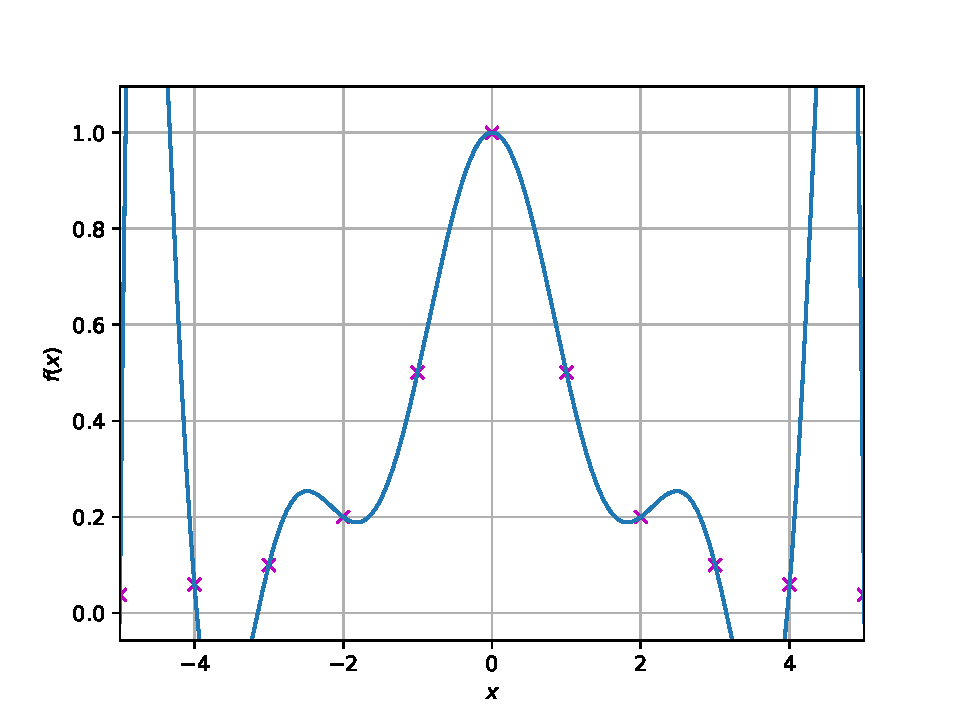
\includegraphics[width=0.35\textwidth]{runge1}&
\hspace*{-0.5cm}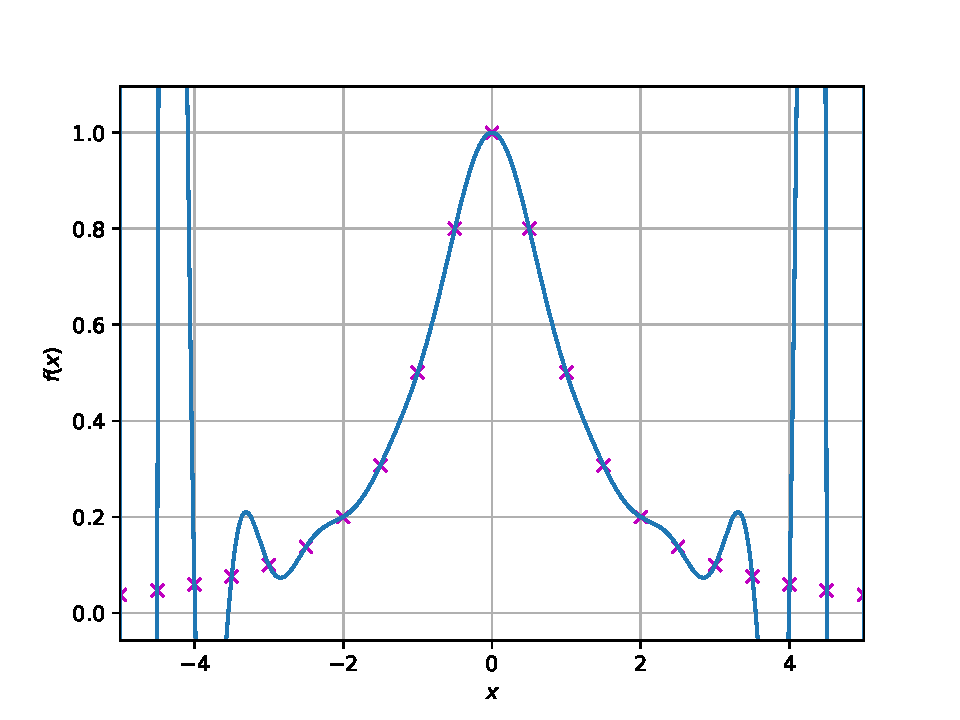
\includegraphics[width=0.35\textwidth]{runge2}&
\hspace*{-0.5cm}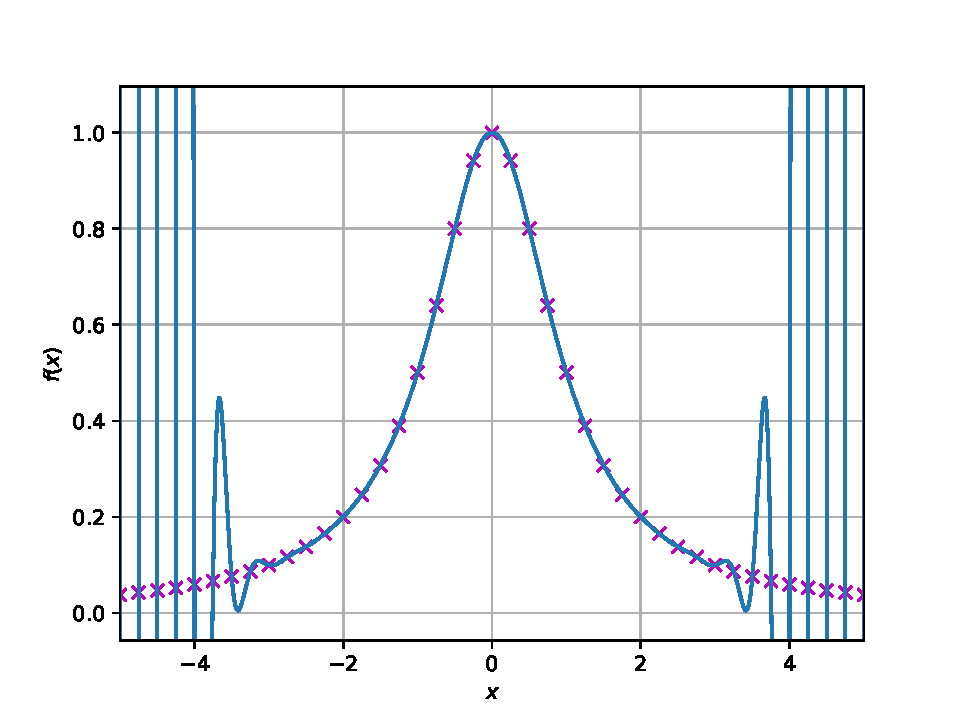
\includegraphics[width=0.35\textwidth]{runge3}\\
(a) & (b) & (c)\\
\end{tabular}
\caption{The Runge phenomenon on interpolating $f(x) = (1+x^2)^{-1}$ on $[-5,5]$: (a) using $11$ equispaced points (b) using $21$ equispaced points (c) using $41$ equispaced points.}
\label{figure:Runge}
\end{center}
\end{figure}

\begin{figure}[htbp]
\begin{center}
\begin{tabular}{ccc}
\hspace*{-0.5cm}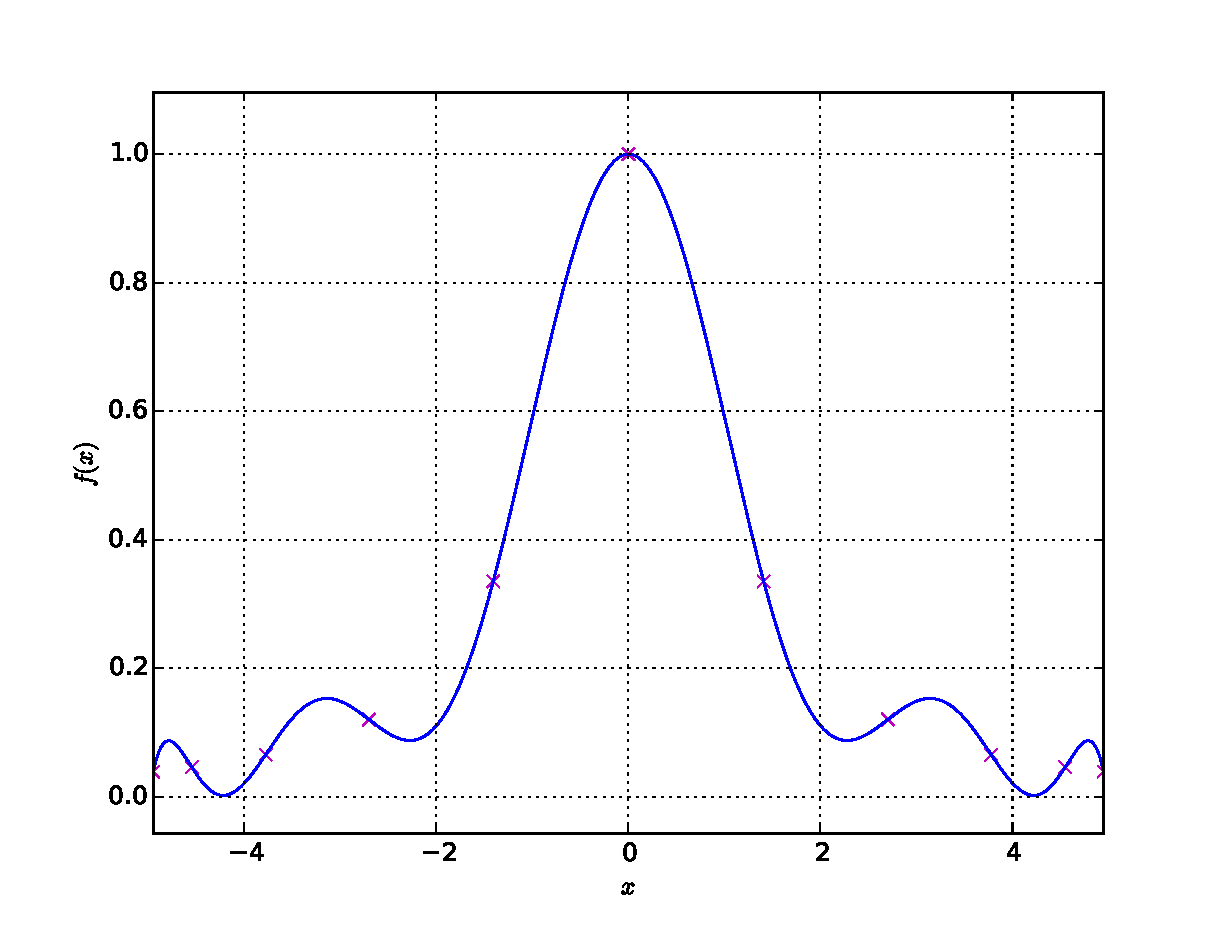
\includegraphics[width=0.35\textwidth]{rungefixed1}&
\hspace*{-0.5cm}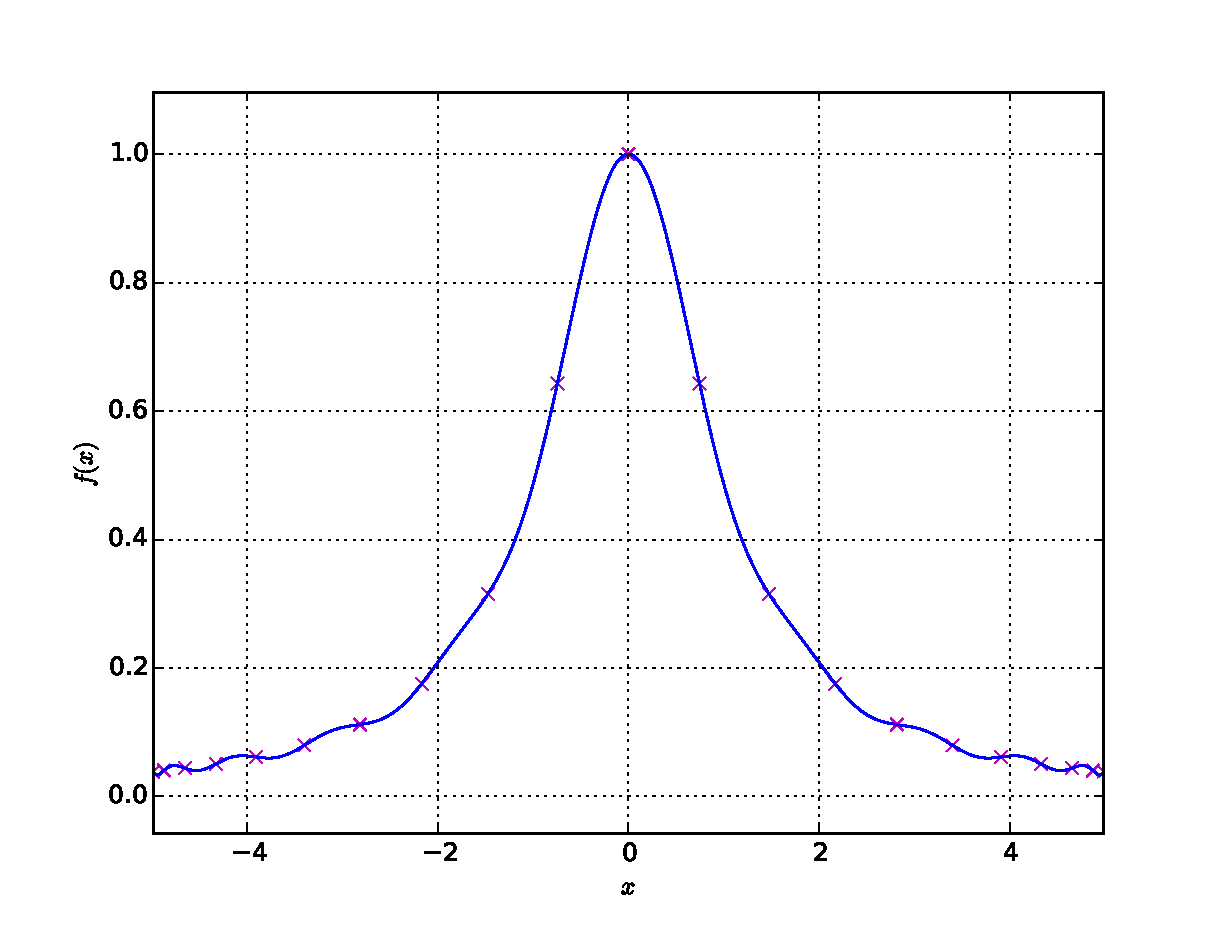
\includegraphics[width=0.35\textwidth]{rungefixed2}&
\hspace*{-0.5cm}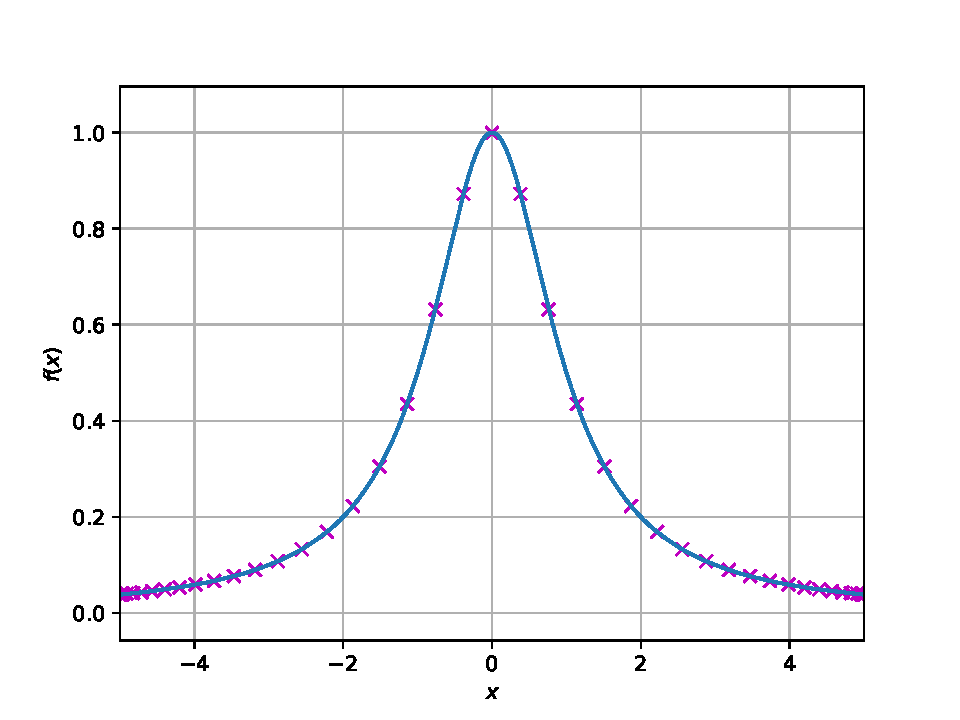
\includegraphics[width=0.35\textwidth]{rungefixed3}\\
(a) & (b) & (c)\\
\end{tabular}
\caption{Uniform convergence on interpolating $f(x) = (1+x^2)^{-1}$ on $[-5,5]$: (a) using $11$ Chebyshev points (b) using $21$ Chebyshev points (c) using $41$ Chebyshev points.}
\label{figure:RungeFixed}
\end{center}
\end{figure}

\section{Best Polynomial Approximation}

Given a function $f:D\to\C$, we wish to find its best polynomial approximation. To measure our progress, we can use $L^p(D,\ud\mu(x))$ spaces and their associated norms: find $p_n\in\P_n$ that is the best polynomial approximation to $f\in L^p(D,\ud\mu(x))$ such that:
\[
\|f-p_n\|_p \le \|f-q\|_p,\qquad\forall q\in\P_n.
\]
Posed in this generality, the problem is still the subject of ongoing research. Therefore, to make any reasonable progress, we will consider the solved problems of best approximation in $L^2$ followed by best approximation in $L^\infty$.

\subsection{Best Polynomial Approximation in $L^2$ and Orthogonal Polynomials}

We now consider the best polynomial approximations in $L^2(D,\ud\mu(x))$, i.e. find $p_n\in\P_n$ such that:
\[
\|f-p_n\|_2 \le \|f-q\|_2,\qquad\forall q\in\P_n.
\]
Supposing $p_n$ has the form $p_n(x) = \sum_{i=0}^n \alpha_i x^i$ then results in the minimization problem:
\[
\min_{(\alpha_0,\ldots,\alpha_n)\in\C^n} \int_D \abs{f(x)-\sum_{i=0}^n \alpha_i x^i}^2\ud\mu(x).
\]
The unique minimizer can be found from the (linear) system:
\[
\dfrac{\partial}{\partial\alpha_k}\int_D \abs{f(x)-\sum_{i=0}^n \alpha_i x^i}^2\ud\mu(x),\quad\hbox{for each}\quad k=0,\ldots,n.
\]
But there is some additional structure that we will exploit rather than solving this system of equations.

\begin{theorem}
If $f\in L^2(D,\ud\mu(x))$ and $p_n\in\P_n$ is such that:
\begin{equation}\label{eq:L2assumption}
\langle r,f-p_n\rangle = 0,\quad \forall r\in\P_n,
\end{equation}
then:
\begin{equation}
\|f-p_n\|_2 \le \|f-r\|_2,\quad \forall r\in\P_n,
\end{equation}
i.e. $p_n$ is a best (weighted) least-squares approximation to $f$ on $D$.
\end{theorem}
\begin{proof}
\begin{align*}
\|f-p_n\|_2^2 & = \abs{\langle f-p_n,f-p_n\rangle}\\
& = \abs{\langle f-r,f-p_n\rangle + \langle r-p_n,f-p_n\rangle},\quad \forall r\in\P_n.
\end{align*}
Since $r-p_n\in\P_n$, the assumption~\eqref{eq:L2assumption} implies that:
\begin{align*}
\|f-p_n\|_2^2 & = \abs{\langle f-r,f-p_n\rangle}\\
& \le \|f-r\|_2\|f-p_n\|_2,
\end{align*}
by the Cauchy--Schwarz inequality.
\end{proof}
\begin{remark}
The converse is also true.
\end{remark}

This gives a direct, albeit poor, way to calculate best polynomial approximations in $L^2$: we wish to find $p_n(x) = \sum_{i=0}^n \alpha_i x^i$ such that:
\begin{equation}
\int_D \conj{x^k}\br[f(x)-\sum_{i=0}^n \alpha_i x^i]\ud\mu(x) = 0,\quad{\rm for}\quad k=0,\ldots,n.
\end{equation}
Rearranging these equations, we have:
\begin{equation}
\sum_{i=0}^n\left(\int_D\conj{x^k}x^i\ud\mu(x)\right)\alpha_i = \int_D \conj{x^k}f(x)\ud\mu(x),\quad{\rm for}\quad k=0,\ldots,n,
\end{equation}
which is the component-wise statement of the matrix equation:
\begin{equation}\label{eq:normalequations}
A\alpha = \varphi,
\end{equation}
to determine the coefficients $\alpha = \pr(\alpha_0,\ldots,\alpha_n)^\top$ from the data $\varphi = \pr(\varphi_0,\ldots,\varphi_n)^\top$, where:
\begin{equation}
A_{k,i} = \int_D \conj{x^k}x^i\ud\mu(x),\quad{\rm and}\quad \varphi_k = \int_D \conj{x^k}f(x)\ud\mu(x).
\end{equation}
The system~\eqref{eq:normalequations} are called the {\bf normal equations}.

\begin{example}
We wish to find the best least-squares approximation to $e^x$ on $[0,1]$ from $\P_1$. We must solve:
\[
\int_0^1 1[e^x -(\alpha_0+\alpha_1x)]\ud x = 0,\quad{\rm and}\quad \int_0^1 x[e^x -(\alpha_0+\alpha_1x)]\ud x = 0.
\]
This is equivalent to:
\begin{align*}
\alpha_0\int_0^1\ud x + \alpha_1\int_0^1x\ud x & = \int_0^1 e^x\ud x,\\
\alpha_0\int_0^1x\ud x + \alpha_1\int_0^1x^2\ud x & = \int_0^1 e^xx\ud x,
\end{align*}
or:
\begin{align*}
\begin{bmatrix}
1 & \frac{1}{2}\\
\frac{1}{2} & \frac{1}{3}\\
\end{bmatrix}
\begin{bmatrix}
\alpha_0\\\alpha_1\\
\end{bmatrix}
\begin{bmatrix}
e-1\\1\\
\end{bmatrix},
\end{align*}
which has the solution $\alpha_0 = 4e-10$ and $\alpha_1 = 18-6e$. Therefore, $p_1(x) = (18-6e)x + (4e-10)$ is the best approximation to $e^x$ in $L^2([0,1],\ud x)$.
\end{example}

\begin{theorem}
The matrix $A$ in~\eqref{eq:normalequations} is nonsingular.
\end{theorem}
\begin{proof}
Suppose $A$ {\em is} singular, i.e. $\exists \alpha\ne 0$ such that $A\alpha = 0$ implying $\alpha^* A\alpha = 0$. This is:
\begin{equation}
\sum_{k=0}^n\conj{\alpha_k}(A\alpha)_k \Longleftrightarrow \sum_{k=0}^n\conj{\alpha_k}\sum_{i=0}^nA_{k,i}\alpha_i = 0.
\end{equation}
Since, by definition $A_{k,i} = \int_D \conj{x^k}x^i\ud\mu(x)$, we find:
\begin{equation}
\Longleftrightarrow \sum_{k=0}^n \conj{\alpha_k} \sum_{i=0}^n \int_D \conj{x^k}x^i\ud\mu(x) \alpha_i = 0.
\end{equation}
Rearranging gives:
\begin{equation}
\int_D\conj{\pr(\sum_{k=0}^n \alpha_kx^k)}\pr(\sum_{i=0}^n \alpha_ix^i)\ud\mu(x) = 0,\quad{\rm or}\quad \left\|\sum_{i=0}^n \alpha_i x^i\right\|_2^2 = 0.
\end{equation}
But this last equality implies that $\sum_{i=0}^n\alpha_ix^i\equiv0$ and thus $\alpha_i\equiv0$ for $i=0,\ldots,n$. We have arrived at a contradiction.
\end{proof}
Invertibility of the matrix $A$ establishes existence and uniqueness of the best polynomial approximation in $L^2(D,\ud\mu(x))$. It does not, however, imply that the normal equations are well-conditioned. To find a well-conditioned solution to this problem, we use our knowledge of the QR factorization for matrices to construct degree-graded polynomial bases that behave significantly better than the monomials.

\begin{example}
Set up, but do not evaluate, the linear system for the best degree-$n$ polynomial approximation in $L^2([0,1],\ud x)$ by using the monomial basis.

The entries of the matrix $A$ are $A_{k,i} = \langle x^k, x^i\rangle = \int_0^1 x^{k+i}\ud x = \dfrac{1}{k+i+1}$, while the right-hand side is $\langle x^k, f\rangle = \int_0^1x^k f(x)\ud x$. In this example, the matrix $A$ turns out to be the notorious Hilbert matrix, whose terrible conditioning we explored in chapter 1.
\end{example}

The solution of the normal equations $A\alpha = \varphi$ for best least-squares polynomial approximation would be trivial if $A$ were diagonal. Instead of using $\{1,x,\ldots,x^n\}$ as a basis for $\P_n$, we shall construct a basis $\{\pi_0,\pi_1,\ldots,\pi_n\}$ in order to diagonalize $A$.

In this basis, our best polynomial approximation $p_n(x) = \sum_{i=0}^n \beta_i\pi_i(x)$, and the normal equations become:
\begin{equation}
\int_D\conj{\pi_k(x)}\br[f(x)-\sum_{i=0}^n\beta_i\pi_i(x)]\ud\mu(x) = 0,\quad{\rm for}\quad k=0,\ldots,n,
\end{equation}
or equivalently:
\[
\sum_{i=0}^n\left(\int_D\conj{\pi_k(x)}\pi_i(x)\ud\mu(x)\right)\beta_i = \int_D\conj{\pi_k(x)}f(x)\ud\mu(x),\quad{\rm for}\quad k=0,\ldots,n,
\]
or:
\begin{equation}
A\beta = \varphi,
\end{equation}
where $\beta = \pr(\beta_0,\ldots,\beta_n)^\top$, $\varphi = \pr(\varphi_0,\ldots,\varphi_n)^\top$ but now:
\begin{equation}
A_{k,i} = \langle \pi_k, \pi_i \rangle = \int_D \conj{\pi_k(x)}\pi_i(x)\ud\mu(x),\quad{\rm and}\quad \varphi_k = \int_D \conj{\pi_k(x)}f(x)\ud\mu(x).
\end{equation}
The matrix $A$ is diagonalized iff:
\[
\langle \pi_k, \pi_i \rangle ~\left\{\begin{array}{ccc} = 0 & \for & i\ne k,\\ \ne 0 & \for & i = k.\end{array}\right.
\]
We can use this (countably infinite) set of conditions to construct the {\bf orthogonal polynomials} with respect to the measure $\ud\mu(x)$. This is known as the Gram--Schmidt procedure.

\begin{lemma} Suppose that $\pi_0,\ldots,\pi_k,$ with $\pi_i\in\P_i$ for each $i$, are orthogonal with respect to the inner product $\langle f,g\rangle = \int_D\conj{f(x)}g(x)\ud\mu(x)$. Then:
\[
\pi_{k+1}(x) = x^{k+1} - \sum_{i=0}^k\delta_i\pi_i(x),
\]
satisfies:
\[
\langle \pi_{j},\pi_{k+1} \rangle = 0,\quad{\rm for}\quad j=0,\ldots,k,\quad{\and}\quad \delta_j = \dfrac{\langle \pi_j,x^{k+1}\rangle}{\langle\pi_j,\pi_j\rangle}.
\]
\end{lemma}
\begin{proof}
For any $j=0,\ldots,k$,
\begin{align*}
\langle\pi_j,\pi_{k+1}\rangle & = \langle \pi_j,x^{k+1}\rangle - \sum_{i=0}^k \delta_i \langle \pi_j,\pi_i\rangle\\
& = \langle \pi_j,x^{k+1}\rangle - \delta_j \langle \pi_j,\pi_j\rangle\quad\hbox{by orthogonality of $\pi_i$ and $\pi_j$ for $i\ne j$},\\
& = 0,\quad\hbox{by definition of $\delta_j$.}
\end{align*}
\end{proof}

\begin{remark}
\begin{enumerate}
\item The Gram--Schmidt procedure constructs orthogonal polynomials inductively starting from $\pi_0(x) = 1$. $\pi_k(x)$ is always of exact degree $k$, so $\{\pi_0,\ldots,\pi_k\}$ is a basis for $\P_k$, $\forall k\in\N_0$. The orthogonal polynomials can be normalized to be {\bf orthonormal}, i.e. $\langle\pi_k,\pi_k\rangle = 1$, to be {\bf monic}, i.e. $\hat{\pi}_k(x) = x^k + \cdots +$, or even have other normalizations such as $\pi_k(1)=1$.
\item The Gram--Schmidt procedure may be organized in a matrix:
\[
\begin{bmatrix}
1\\
\frac{\langle \pi_0, x\rangle}{\langle \pi_0,\pi_0\rangle} & 1\\
\frac{\langle \pi_0, x^2\rangle}{\langle \pi_0,\pi_0\rangle} & \frac{\langle \pi_1, x^2\rangle}{\langle \pi_1,\pi_1\rangle} & 1\\
\frac{\langle \pi_0, x^3\rangle}{\langle \pi_0,\pi_0\rangle} & \frac{\langle \pi_1, x^3\rangle}{\langle \pi_1,\pi_1\rangle} & \frac{\langle \pi_2, x^3\rangle}{\langle \pi_2,\pi_2\rangle} & 1\\
\vdots & \vdots & \cdots & \cdots & \ddots\\
\frac{\langle \pi_0, x^n\rangle}{\langle \pi_0,\pi_0\rangle} & \frac{\langle \pi_1, x^n\rangle}{\langle \pi_1,\pi_1\rangle} & \cdots & \cdots & \frac{\langle \pi_{n-1}, x^n\rangle}{\langle \pi_{n-1},\pi_{n-1}\rangle} & 1\\
\end{bmatrix}
\begin{bmatrix}
\pi_0(x)\\\pi_1(x)\\\pi_2(x)\\\pi_3(x)\\\vdots\\\pi_n(x)
\end{bmatrix}
=
\begin{bmatrix}
1\\x\\x^2\\x^3\\\vdots\\x^n
\end{bmatrix},
\]
where the system is solved by $\OO(n^2)$ inner products and forward substitution with $\OO(n^2)$ flops. Entries in subsequent rows are computed on-the-fly, once the required orthogonal polynomials are known.
\end{enumerate}
\end{remark}

\subsubsection{Properties of Orthogonal Polynomials}

In order to provide a basis for computational techniques associated with the preceding approximations, as well as for later developments, we next exhibit some useful properties of orthogonal polynomials.

\begin{theorem}\label{theorem:OPzeros}
For every $n\in\N$ and $a,b\in\R$, if the measure $\mu$ is monotonic, the orthogonal polynomials $\pi_n$ with respect to $L^2([a,b],\ud\mu(x))$ possess $n$ distinct real zeros contained in $(a,b)$.
\end{theorem}
\begin{proof}
If $\pi_n$ does not change in sign in $[a,b]$, then:
\[
\int_a^b\pi_n\ud\mu(x) = \langle \pi_0,\pi_n\rangle,
\]
is either positive or negative. In either case, this is a contradiction since the right-hand side must be zero by orthogonality. Hence, $\pi_n$ must have a zero in $(a,b)$. Now, let those real zeros of $\pi_n(x)$ which are of {\em odd} multiplicity, and which lie in $(a,b)$, be denoted by $x_1, x_2,\ldots, x_m,$ and {\em assume} that $m<n$. Then the product:
\[
(x-x_1)(x-x_2)\cdots(x-x_m)\pi_n(x),
\]
does not change sign in $[a,b]$. Since $m<n$, the product $(x-x_1)\cdots(x-x_m)$ is a polynomial of degree less than $n$ and it may be expressed in terms of the basis $\{\pi_k(x)\}_{k=0}^m$. We must have:
\begin{equation}\label{eq:MonotonicOP}
\langle (x-x_1)(x-x_2)\cdots(x-x_m),\pi_n(x)\rangle = 0.
\end{equation}
However, since the measure is monotonic in $[a,b]$, the integrand therefore has the same property, and we have reached a contradiction, as this guarantees that~\eqref{eq:MonotonicOP} must be different from $0$. Hence, it follows that $m=n$, and since the total multiplicity of {\em all} zeros is equal to $n$, all roots must be real and distinct and must lie in $(a,b)$.
\end{proof}

\begin{theorem}\label{theorem:threetermrecurrence}
For every $n\in\N$, the monic orthogonal polynomials $\hat{\pi}_n$ with respect to $L^2([a,b],\ud\mu(x))$ satisfy a three-term recurrence relation of the form:
\begin{equation}\label{eq:threetermrecurrence}
\hat{\pi}_{n+1}(x) = (x-\alpha_n)\hat{\pi}_n(x) - \beta_n\hat{\pi}_{n-1}(x).
\end{equation}
\end{theorem}
\begin{proof}
The case $n=1$ holds trivially. Assume the result holds for $n-1$. Since $\hat{\pi}_{n+1}-x\hat{\pi}_n\in\P_n$ and since $\{\hat{\pi}_0,\ldots,\hat{\pi}_n\}$ is a basis for $\P_n$, it follows that:
\[
\hat{\pi}_{n+1}(x) - x\hat{\pi}_n(x) = -\alpha_n\hat{\pi}_n(x) - \beta_n\hat{\pi}_{n-1} - \sum_{j=0}^{n-2}\gamma_j\hat{\pi}_j(x),
\]
for some constants $\alpha_n$, $\beta_n$, and $\gamma_j$. If we take the inner product with $\hat{\pi}_n$, we obtain:
\[
0 - \langle x\hat{\pi}_n,\hat{\pi}_n\rangle = -\alpha_n\langle\hat{\pi}_n,\hat{\pi}_n\rangle \quad{\rm or}\quad \alpha_n = \dfrac{\langle x\hat{\pi}_n,\hat{\pi}_n\rangle}{\langle\hat{\pi}_n,\hat{\pi}_n\rangle}.
\]
Next, if we take the inner product with $\hat{\pi}_{n-1}$, we obtain:
\[
0 - \langle x\hat{\pi}_n,\hat{\pi}_{n-1}\rangle = -\beta_n\langle\hat{\pi}_{n-1},\hat{\pi}_{n-1}\rangle \quad{\rm or}\quad \beta_n = \dfrac{\langle x\hat{\pi}_n,\hat{\pi}_{n-1}\rangle}{\langle\hat{\pi}_{n-1},\hat{\pi}_{n-1}\rangle} = \dfrac{\langle \hat{\pi}_n,x\hat{\pi}_{n-1}\rangle}{\langle\hat{\pi}_{n-1},\hat{\pi}_{n-1}\rangle} = \dfrac{\langle \hat{\pi}_n,\hat{\pi}_n\rangle}{\langle\hat{\pi}_{n-1},\hat{\pi}_{n-1}\rangle}.
\]
Finally, any of the inner products with $\hat{\pi}_j$ for $j=0,\ldots,n-2$ give:
\[
0 - \langle x\hat{\pi}_n,\hat{\pi}_{j}\rangle = -\gamma_j\langle\hat{\pi}_{j},\hat{\pi}_{j}\rangle.
\]
Since $\deg(x\hat{\pi}_j) = j+1 < n$, each of the $\gamma_j=0$.
\end{proof}

Without loss of generality, orthogonal polynomials $\pi_n$ with any normalization (not necessarily monic) satisfy a three-term recurrence relation. Consider then the notation:
\begin{equation}\label{eq:OPrec}
\pi_{n+1}(x) = (A_nx+B_n)\pi_n(x) -C_n\pi_{n-1}(x),\qquad \pi_{-1}(x) = 0,\quad \pi_0(x) = 1.
\end{equation}
The following algorithm is the extension of Horner's rule for numerical evaluation of polynomials expressed in general orthogonal polynomial bases. The Clenshaw--Smith algorithm writes the sum:
\begin{equation}
p_n(x) = \sum_{k=0}^n c_k \pi_k(x),
\end{equation}
via an inhomogeneous recurrence relation involving the adjoint of~\eqref{eq:OPrec} as follows:
\begin{algorithm}[Clenshaw--Smith~\cite{Clenshaw-9-118-55,Smith-19-33-65}]~
\begin{enumerate}
\item Set:
\begin{equation}
u_{n+1}(x) = u_{n+2}(x) = 0.
\end{equation}
\item For $k=n,n-1,\ldots,0$:
\begin{equation}
u_k(x) = (A_kx+B_k)u_{k+1}(x) - C_{k+1}u_{k+2}(x) + c_k.
\end{equation}
\item Then:
\begin{equation}
p_n(x) = u_0(x).
\end{equation}
\end{enumerate}
\end{algorithm}

The Clenshaw--Smith allows for numerical evaluation of polynomials expressed in orthogonal bases in $\OO(n)$ flops with $\OO(1)$ storage.

\begin{theorem}\label{theorem:ChristoffelDarboux}
Let $\tilde{\pi}_n$ represent the orthonormal polynomials with respect to $L^2([a,b],\ud\mu(x))$. Then, the Christoffel--Darboux formula is:
\begin{equation}\label{eq:ChristoffelDarboux}
\sum_{k=0}^{n-1}\tilde{\pi}_k(x)\tilde{\pi}_k(y) = \sqrt{\beta_n}\dfrac{\tilde{\pi}_n(x)\tilde{\pi}_{n-1}(y) - \tilde{\pi}_{n-1}(x)\tilde{\pi}_n(y)}{x-y}.
\end{equation}
\end{theorem}
\begin{proof}
Multiplying the three-term recurrence relation~\eqref{eq:threetermrecurrence} by $\hat{\pi}_k(y)$ and subtracting the resulting relation from the one with $x$ and $y$ interchanged yields:
\[
(x-y)\hat{\pi}_k(x)\hat{\pi}_k(y) = \beta_k\hat{\pi}_{k-1}(x)\hat{\pi}_k(y) - \beta_k \hat{\pi}_k(x)\hat{\pi}_{k-1}(y) + \hat{\pi}_{k+1}(x)\hat{\pi}_k(y) - \hat{\pi}_k(x)\hat{\pi}_{k+1}(y).
\]
Recall that $\beta_k = \frac{\langle \hat{\pi}_k,\hat{\pi}_k\rangle}{\langle\hat{\pi}_{k-1},\hat{\pi}_{k-1}\rangle}$. So this relation is equivalent to:
\begin{align*}
(x-y)\dfrac{\hat{\pi}_k(x)\hat{\pi}_k(y)}{\langle \hat{\pi}_k,\hat{\pi}_k\rangle} & = \dfrac{\hat{\pi}_{k-1}(x)\hat{\pi}_k(y)}{\langle\hat{\pi}_{k-1},\hat{\pi}_{k-1}\rangle} - \dfrac{\hat{\pi}_k(x)\hat{\pi}_{k-1}(y)}{\langle\hat{\pi}_{k-1},\hat{\pi}_{k-1}\rangle}\\ & - \dfrac{\hat{\pi}_k(x)\hat{\pi}_{k+1}(y)}{\langle \hat{\pi}_k,\hat{\pi}_k\rangle} + \dfrac{\hat{\pi}_{k+1}(x)\hat{\pi}_k(y)}{\langle \hat{\pi}_k,\hat{\pi}_k\rangle}.
\end{align*}
Summing both sides from $k=0$ to $k=n-1$ and observing $\hat{\pi}_{-1}\equiv0$ and the telescoping nature of the summation on the right gives:
\[
\sum_{k=0}^{n-1} \dfrac{\hat{\pi}_k(x)\hat{\pi}_k(y)}{\langle \hat{\pi}_k,\hat{\pi}_k\rangle} = \dfrac{1}{\langle \hat{\pi}_{n-1},\hat{\pi}_{n-1}\rangle} \dfrac{\hat{\pi}_n(x)\hat{\pi}_{n-1}(y) - \hat{\pi}_{n-1}(x)\hat{\pi}_n(y)}{x-y}.
\]
Equation~\eqref{eq:ChristoffelDarboux} only requires orthonormalization.
\end{proof}

\subsubsection{The Classical Orthogonal Polynomials}

The classical orthogonal polynomials are all eigenfunctions of linear second-order homogeneous differential equations of the form:
\begin{equation}
Q(x)\pi_n''(x) + L(x)\pi_n'(x) = \lambda_n\pi_n(x),
\end{equation}
where $Q\in\P_2$ and $L\in\P_1$, and where the eigenvalues are given by $\lambda_n = nL'(x) +\dfrac{n(n-1)}{2}Q''(x)$. With this extra structure, an explicit representation in terms of higher order derivatives can be derived.
\begin{theorem}[p. 24 of Nikiforov and Uvarov~\cite{Nikiforov-Uvarov-88}]\label{theorem:Rodrigues}
The classical orthogonal polynomials $\pi_n\in\P_n$ with respect to the inner product space $L^2(D,w(x)\ud x)$ can be expressed by {\bf Rodrigues' formula}:
\begin{equation}
\pi_n(x) = \dfrac{1}{\kappa_n w(x)}\dfrac{\ud^n}{\ud x^n}\left(w(x)(Q(x))^n\right).
\end{equation}
\end{theorem}

\begin{example}
The Legendre polynomials, denoted by $P_n(x)$, are orthogonal with respect to $L^2(\I,\ud x)$ and are normalized by $P_n(1)=1$. They satisfy the differential equation:
\begin{equation}
(1-x^2)\pi_n''(x) -2x\pi_n'(x) + n(n+1)\pi_n(x) = 0,
\end{equation}
and therefore, Rodrigues' formula states that:
\begin{equation}
P_n(x) = \dfrac{1}{(-2)^nn!}\dfrac{\ud^n}{\ud x^n}\left(1-x^2\right)^n.
\end{equation}
\end{example}

\begin{example}
The Chebyshev polynomials of the first kind, denoted by $T_n(x)$, are orthogonal with respect to $L^2(\I,(1-x^2)^{-\frac{1}{2}}\ud x)$ and are normalized by $T_n(1)=1$. By making the variable transformation $x=\cos\theta$, the inner product becomes:
\[
\langle \pi_k,\pi_j\rangle = \int_0^\pi \pi_k(\cos\theta)\pi_j(\cos\theta)\ud\theta.
\]
Explicitly:
\begin{equation}\label{eq:Tn}
T_n(\cos\theta) = \cos(n\theta),\quad{\rm or}\quad T_n(x) = \cos(n\cos^{-1}(x)).
\end{equation}
\end{example}

\begin{example}
The Chebyshev polynomials of the second kind, denoted by $U_n(x)$, are orthogonal with respect to $L^2(\I,\sqrt{1-x^2}\ud x)$ and normalized by $U_n(1)=n+1$. By making the variable transformation $x=\cos\theta$, the inner product becomes:
\[
\langle \pi_k,\pi_j\rangle = \int_0^\pi \pi_k(\cos\theta)\pi_j(\cos\theta)\sin^2\theta\ud\theta.
\]
Explicitly:
\begin{equation}
U_n(\cos\theta) = \dfrac{\sin((n+1)\theta)}{\sin\theta},\quad{\rm or}\quad U_n(x) = \dfrac{\sin((n+1)\cos^{-1}(x))}{\sqrt{1-x^2}}.
\end{equation}
\end{example}

Table~\ref{table:ClassicalOrthogonalPolynomials} describes the classical orthogonal polynomials. Note that Legendre and Chebyshev polynomials are special cases of Jacobi polynomials. Figure~\ref{figure:TUP} shows the first six polynomials $T_n(x)$, $U_n(x)$, and $P_n(x)$.

\begin{table}[htp]
\caption{The classical orthogonal polynomials}
\begin{center}
\begin{tabular}{cccc}
\sphline
Name & Jacobi & Laguerre & Hermite\\
\sphline
Notation & $P_n^{(\alpha,\beta)}(x)$ & $L_n(x)$ & $H_n(x)$\\
\sphline
Domain & $\I$ & $[0,\infty)$ & $\R$\\
\sphline
$w(x)$ & $(1-x)^\alpha(1+x)^\beta$ & $e^{-x}$ & $e^{-x^2}$\\
$A_n$ & $\dfrac{(2n+\alpha+\beta+1)(2n+\alpha+\beta+2)}{2(n+1)(n+\alpha+\beta+1)}$ & $-\dfrac{1}{n+1}$ & $2$\\
$B_n$ & $\dfrac{(\alpha^2-\beta^2)(2n+\alpha+\beta+1)}{2(n+1)(n+\alpha+\beta+1)(2n+\alpha+\beta)}$ & $\dfrac{2n+1}{n+1}$ & $0$\\
$C_n$ & $\dfrac{(n+\alpha)(n+\beta)(2n+\alpha+\beta+2)}{(n+1)(n+\alpha+\beta+1)(2n+\alpha+\beta)}$ & $\dfrac{n}{n+1}$ & $2n$\\
$Q(x)$ & $1-x^2$ & $x$ & $1$\\
$\kappa_n$ & $(-2)^nn!$ & $n!$ & $(-1)^n$\\
\sphline
\end{tabular}
\end{center}
\label{table:ClassicalOrthogonalPolynomials}
\end{table}%

\begin{figure}[htbp]
\begin{center}
\begin{tabular}{ccc}
\hspace*{-0.5cm}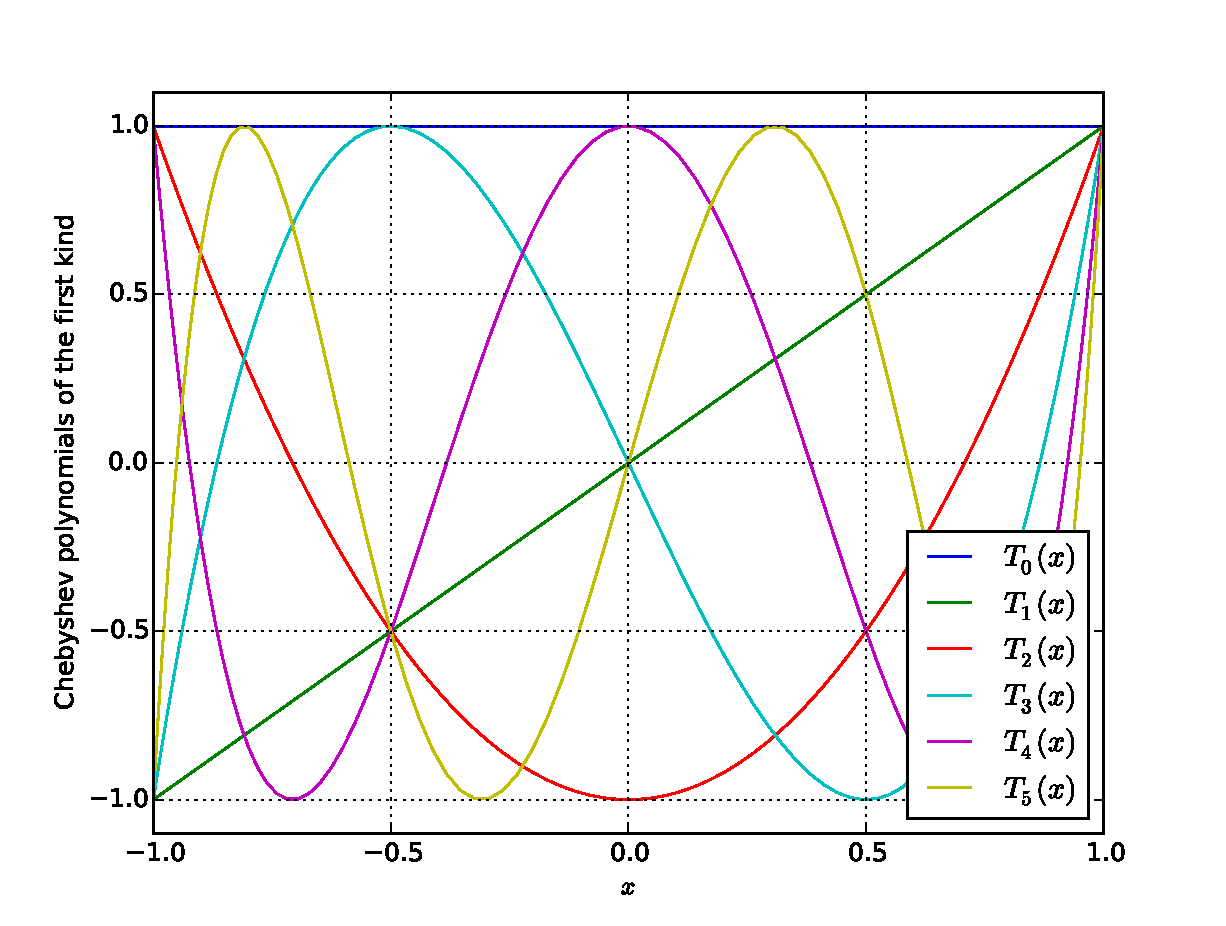
\includegraphics[width=0.35\textwidth]{chebyshevt}&
\hspace*{-0.5cm}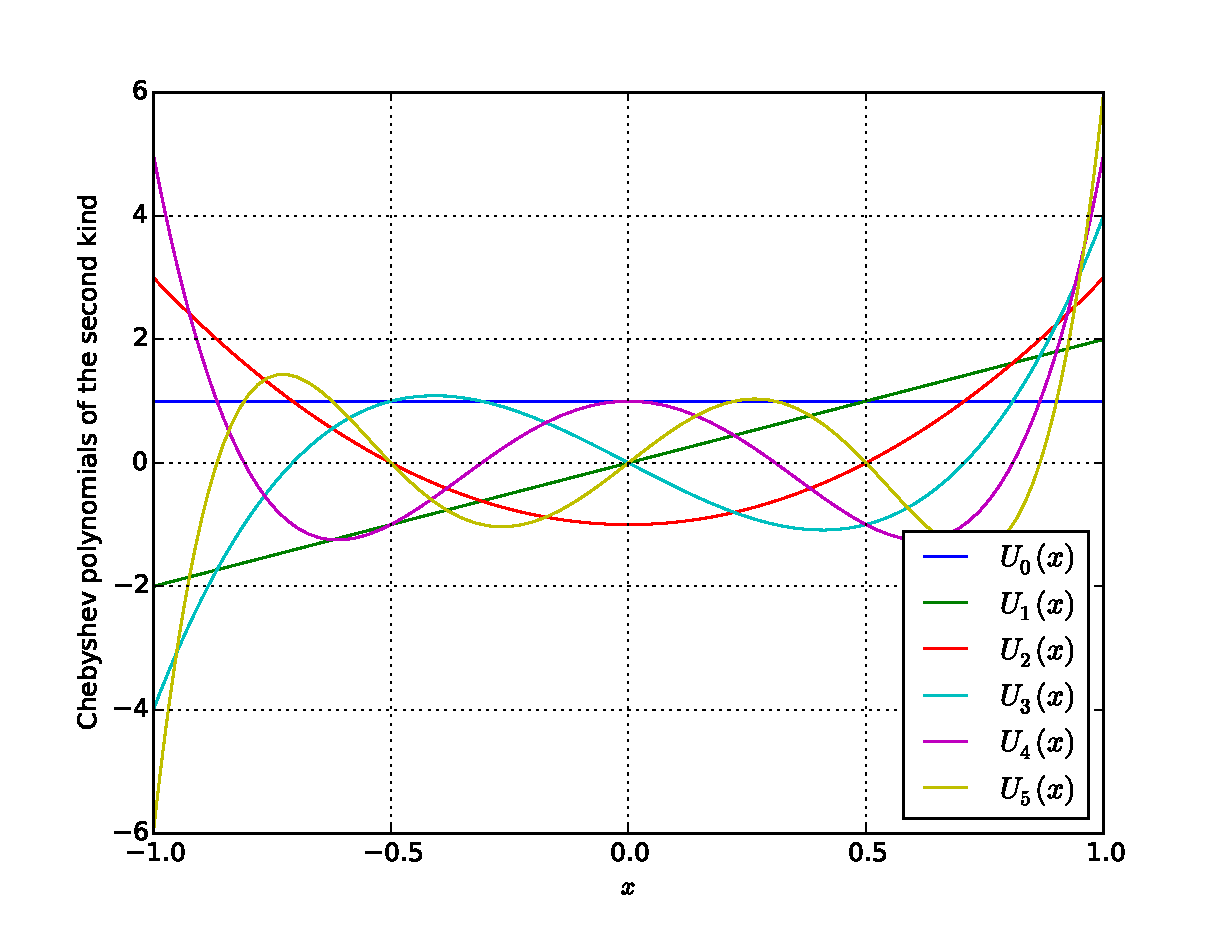
\includegraphics[width=0.35\textwidth]{chebyshevu}&
\hspace*{-0.5cm}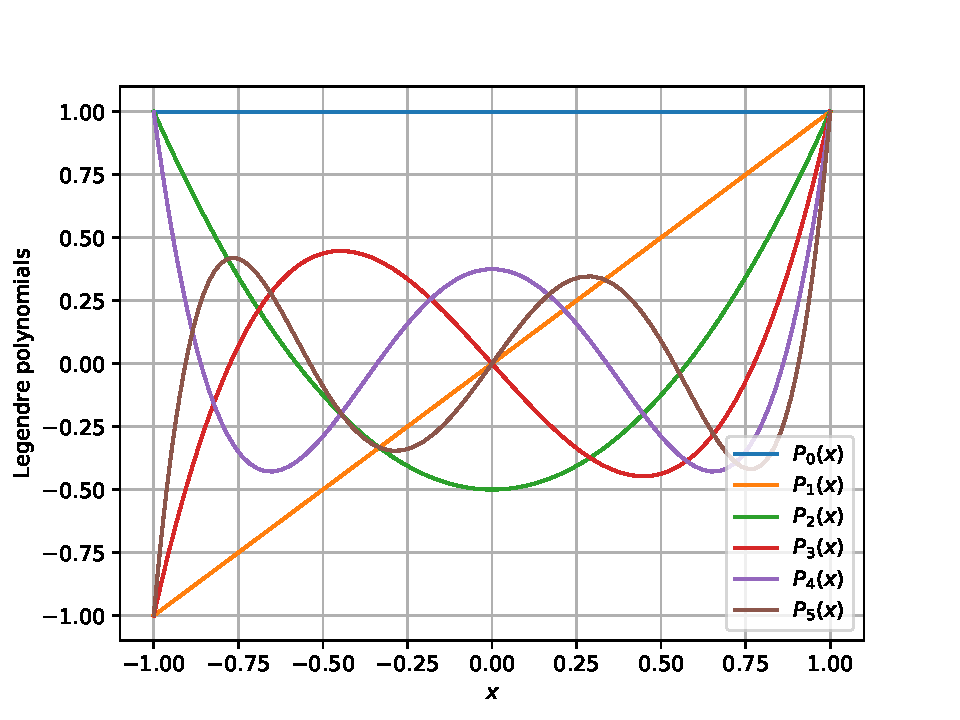
\includegraphics[width=0.35\textwidth]{legendre}\\
(a) & (b) & (c)\\
\end{tabular}
\caption{The first six Chebyshev polynomials of the (a) first kind, (b) second kind, and (c) Legendre polynomials.}
\label{figure:TUP}
\end{center}
\end{figure}

\subsection{Best Polynomial Approximation in $L^\infty$ and The Remez Exchange Algorithm}

We have seen that best polynomial approximation in $L^2$ is a rich and well-developed subject. Best polynomial approximation in $L^\infty$ is just as fascinating, though as the results will show, it is hardly as practical. It turns out that best polynomial approximation in $L^\infty$ is an old idea dating from the time of Chebyshev and Poncelet.

In this section, we consider the best polynomial approximations in $L^\infty([a,b])$, i.e. find $p_n\in\P_n$ such that:
\[
\|f-p_n\|_\infty \le \|f-q\|_\infty,\qquad\forall q\in\P_n.
\]
The main result of this section is to characterize the polynomials of best approximation as {\bf alternants}.
\begin{theorem}[Chap.~10 in Trefethen~\cite{Trefethen-12}]\label{theorem:Equioscillation}
Every $f\in C([a,b])$ has a unique best approximation $p_n\in\P_n$. If $f$ is real, then $p_n$ is real, and in this case a polynomial $q\in\P_n$ is equal to $p_n$ if and only if $f-q$ equioscillates in at least $n+2$ extreme points.
\end{theorem}
\begin{proof}
We partition the proof.
\begin{description}
\item[Existence] We note that $\|f-q\|_\infty$ is a continuous function of $q\in\P_n$. Since one candidate approximation is the zero function, we know that if $p_n$ exists, it lies in $\{q\in\P_n : \|f-q\|_\infty \le \|f\|_\infty\}$. This is a closed and bounded subset of a finite-dimensional space, hence compact (the Heine--Borel theorem), and thus the minimum is attained.
\item[Equioscillation $\Longrightarrow$ optimality] Suppose $f$ and $p$ are real and $(f-p)(x)$ takes equal extreme values with alternating signs at $n+2$ points $x_0<\cdots<x_{n+1}$, and suppose $\|f-q\|_\infty < \|f-p\|_\infty$ for some real polynomial $q\in\P_n$. Then $p-q$ must take nonzero values with alternating signs at the equisocillation points, implying that it takes the value zero in at least $n+1$ points in between. This implies that $p-q\equiv0$, which is a contradiction.
\item[Optimality $\Longrightarrow$ equioscillation] Suppose $f-p$ equioscillates at fewer than $n+2$ points, and set $e = \|f-p\|_\infty$. Without loss of generality, suppose the leftmost extremum is one where $f-p = -e$. Then there are numbers $a < x_1 < \cdots < x_k < b$ with $k\le n$ such that $(f-p)(x) < e$ for $x\in[a,x_1]\cup[x_2,x_3]\cup[x_4,x_5]\cup\cdots\cup$ and $(f-p)(x)>-e$ for $x\in[x_1,x_2]\cup[x_3,x_4]\cup\cdots\cup$. If we define $\delta p(x) := (x_1-x)(x_2-x)\cdots(x_k-x)$, then $(p-\varepsilon\delta p)(x)$ will be a better approximation than $p$ to $f$ for all sufficiently small $\varepsilon>0$.
\item[Uniqueness] Suppose $p$ is a best approximation with equioscillation extrema $x_0<x_1<\cdots<x_{n+1}$, and suppose $\|f-q\|_\infty \le \|f-p\|_\infty$ for some real polynomial $q\in\P_n$. Then, without loss of generality, $(p-q)(x)$ must be nonpositive at $x_0,x_2,x_4,\ldots,$ and nonnegative at $x_1,x_3,x_5,\ldots.$ This implies that $p-q$ has roots in each of the $n+1$ closed intervals $[x_0,x_1], [x_1,x_2],\ldots,[x_n,x_{n+1}]$. We wish to conclude that $p-q$ has at least $n+1$ roots in total, counted with multiplicity, implying that $p=q$. To make the argument we prove by induction that $p-q$ has at least $k$ roots in $[x_0,x_k]$ for each $k$. The case $k=1$ is immediate. For the general case, suppose that $p-q$ has at least $j$ roots in $[x_0,x_j]$ for each $j\le k-1$ but only $k-1$ roots in $[x_0,x_k]$. Then there must be a simple root at $x_{k-1}$. By the induction hypothesis, $p-q$ must have exactly $k-2$ roots in $[x_0,x_{k-2}]$ with a simple root at $x_{k-2}$, $k-3$ roots in $[x_0,x_{k-3}]$ with a simple root at $x_{k-3}$, and so on down to one root in $[x_0,x_1]$, with a simple root at $x_1$. It follows that $p-q$ must be nonzero at $x_0$ and at $x_k$, and since the sign of $p-q$ changes at each of the simple roots $x_1,\ldots,x_{k-1},$ the signs at $x_0$ and $x_k$ must be the same if $k$ is odd and opposite if $k$ is even. On the other hand, from the original alternation condition, we know that $p-q$ must take the same signs at $x_0$ and at $x_k$ if $k$ is even and opposite signs if $k$ is odd.
\end{description}
\end{proof}

Theorem~\ref{theorem:Equioscillation} provides the mathematical foundation for the Remez exchange algorithm, the algorithm that iteratively computes best polynomial approximations in $L^\infty([a,b])$.

\begin{algorithm}\label{algorithm:Remez} The Remez exchange algorithm on $[-1,1]$. Let $p_n(x) = \sum_{k=0}^n c_kT_k(x)$.
\begin{enumerate}
\item Given the points $-1\le x_0<\cdots<x_{n+1}\le1$, solve the linear system of $n+2$ equations:
\[ c_0 + c_1 T_1(x_i) + \cdots + c_nT_n(x_i) + (-1)^ie = f(x_i)\quad{\rm for}\quad i=0,\ldots,n+1,
\]
for the unknowns $c_0,\ldots,c_n$ and $e$.
\item Improve upon the points $x_0<\cdots<x_{n+1}$ and their errors $\pm e$ by finding the local maxima:
\[
\bar{x}_k = \argmax_{x\in(x_{k-1},x_{k+1})}|f(x)-p_n(x)|,\quad{\rm for}\quad k=1,\ldots,n,
\]
and expect $x_0=a$ and $x_{n+1}=b$.
\item Define $z_i := |f(\bar{x}_i)-p_n(\bar{x}_i)|$ for $i=0,\ldots,n+1$. Then with $z_{\min} := \min\{z_i\}$ and $z_{\max} := \max\{z_i\}$ as lower and upper bounds for the best approximation errors, iterate until $z_{\min} \approx z_{\max}$ in the working precision.
\end{enumerate}
\end{algorithm}
The best polynomial approximation is represented in the basis of the Chebyshev polynomials of the first kind so as to render the system as well-conditioned as possible. A simple variable transformation allows for the algorithm to be applied to the general interval $[a,b]$. The Chebyshev nodes are a common choice for the initial set of points because Chebyshev polynomial interpolants give near-best polynomial approximants in $L^\infty([-1,1])$.

Figure~\ref{figure:Remez} shows the approximants generated by the Remez algorithm to the continuous function $f(x) = |x+\tfrac{1}{2}|$.

\begin{figure}[htbp]
\begin{center}
\begin{tabular}{cc}
\hspace*{-0.5cm}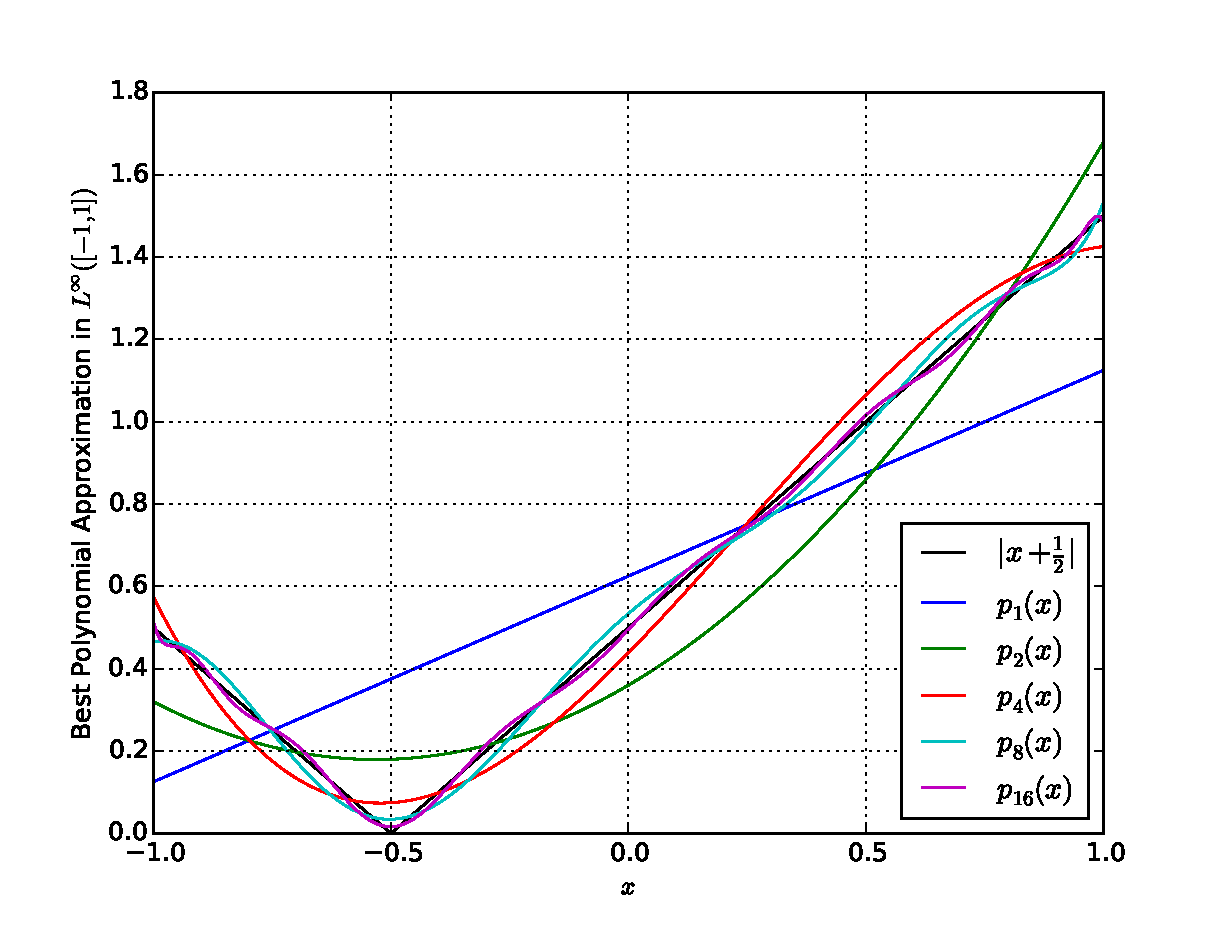
\includegraphics[width=0.525\textwidth]{BPAabs}&
\hspace*{-0.5cm}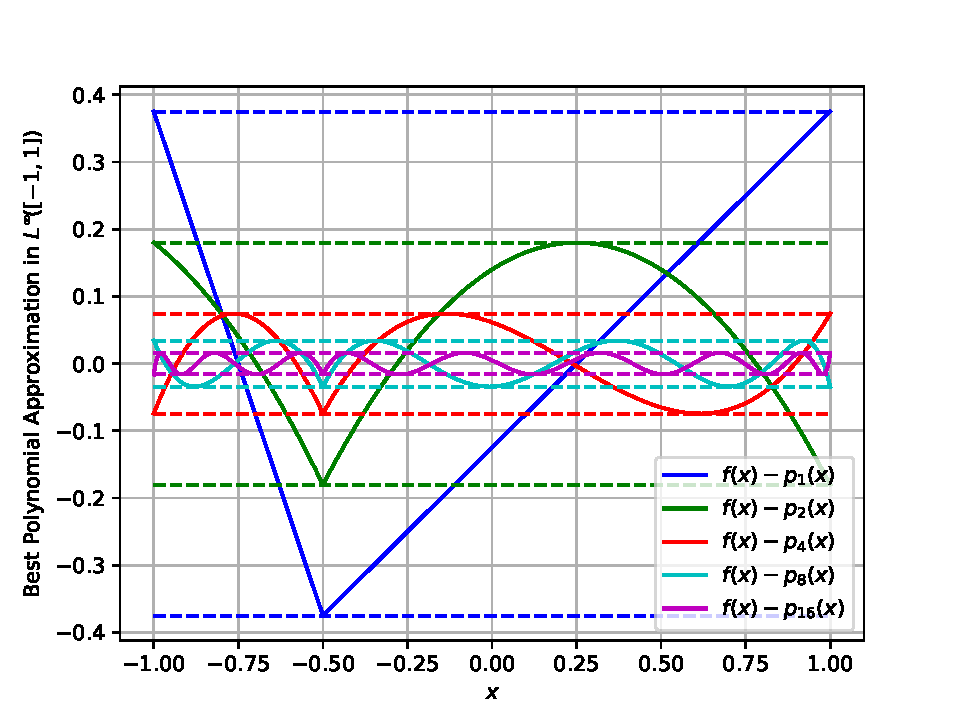
\includegraphics[width=0.525\textwidth]{BPAerrabs}\\
(a) & (b)\\
\end{tabular}
\caption{The Remez algorithm for best polynomial approximation to the continuous function $f(x) = |x+\tfrac{1}{2}|$ on $[-1,1]$: (a) the function and the polynomial approximants (b) the error, showing equioscillation.}
\label{figure:Remez}
\end{center}
\end{figure}


\subsection{The Best Choice of Interpolation Nodes on $\I$}\label{subsection:ChebyshevPointsAreTheBest}

We have now studied Lagrange interpolation; we have seen how best polynomial approximation in $L^2$ leads to the beautiful theory of orthogonal polynomials; and, we have examined the more complicated task of best polynomial approximation in $L^\infty$. We now have all the necessary tools to eliminate the Runge phenomenon that was depicted in Figure~\ref{figure:Runge}. Given the remainder Theorem~\ref{theorem:LagrangeInterpolatingRemainder}, we know that for sufficiently smooth functions, the remainder is given by:
\[
r(x) = f(x)-p_n(x) = \ell(x)\dfrac{f^{(n+1)}(\xi)}{(n+1)!}.
\]
In an effort to obtain uniformly convergent interpolating polynomials, one may ask how best to choose the interpolation points $x_0,\ldots,x_n$. Since the function $\ell(x) = \prod_{i=0}^n(x-x_i)$, we may ask which set of points will minimize the uniform norm:
\[
\inf_{(x_0,\ldots,x_n)\in\I}\|\ell\|_\infty?
\]
This question is answered by the following theorem.
\begin{theorem}
The Chebyshev points of the first kind (i.e. the roots of $T_{n+1}(x)$) infimize $\|\ell\|_\infty$ on $\I$.
\end{theorem}
\begin{proof}
From~\eqref{eq:Tn}, it is clear that the Chebyshev polynomials of the first kind have unit uniform norm, $\|T_{n+1}\|_\infty = 1$. Furthermore, they {\em equioscillate} between their $n+2$ extrema. Invoking Theorem~\ref{theorem:Equioscillation}, we now see that $T_{n+1}$ are the errors associated with {\em best polynomial approximations} (for example, $f(x) = x^{n+1}$ and $p_n(x) = x^{n+1}-2^{-n}T_{n+1}(x)$), and thus infimize the norm. Since $\ell(x)$ is monic, and since the coefficient of $x^{n+1}$ in $T_{n+1}$ is $2^n$ (using induction on the recurrence relations), then:
\[
\inf_{(x_0,\ldots,x_n)\in\I}\|\ell\|_\infty = \|2^{-n}T_{n+1}\|_\infty = 2^{-n},
\]
and the points:
\[
x_k = \cos\left(\dfrac{k+\frac{1}{2}}{n+1}\pi\right),\quad{\rm for}\quad k=0,\ldots,n.
\]
are the roots of $T_{n+1}(x)$.
\end{proof}
Using the Chebyshev points of the first kind as interpolation points leads to the drastic improvement of Figure~\ref{figure:RungeFixed}, and furthermore the uniform approximation bound:
\[
\|f-p_n\|_\infty \le \dfrac{\|f^{(n+1)}\|_\infty}{2^{n}(n+1)!}.
\]

\section{Spline Approximation}

Sometimes a global approximation such as a Lagrange interpolant is not appropriate. For example, if we must sample data at equispaced points, there is no escaping the Runge phenomenon via the selection of a different set of points. In other scenarios, data will be just too ``rough'' to be interpolated efficiently with a global interpolant, shown in Figure~\ref{figure:SplineIntro}.

\begin{figure}[htbp]
\begin{center}
\begin{tabular}{cc}
\hspace*{-0.5cm}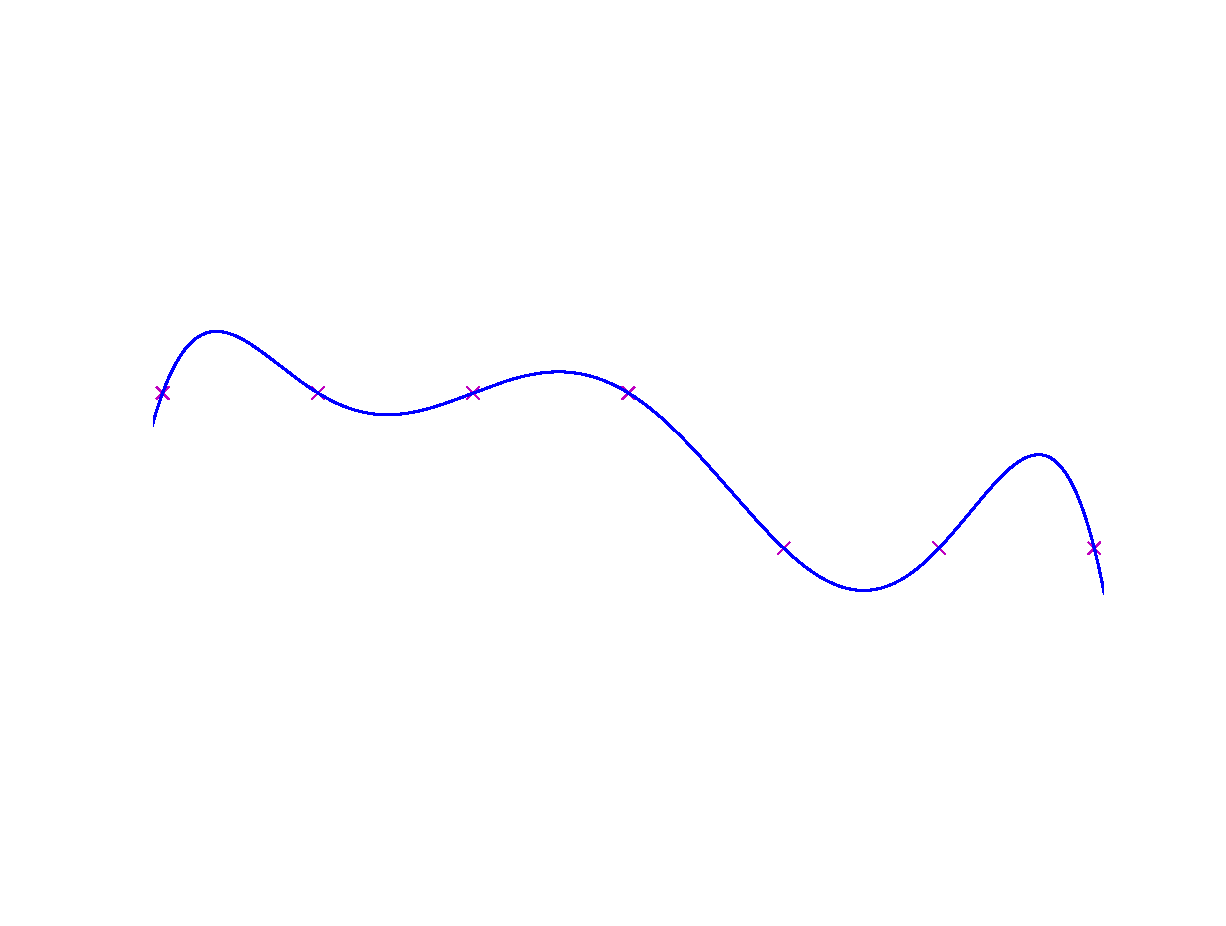
\includegraphics[width=0.45\textwidth]{spline1a}&
\hspace*{-0.5cm}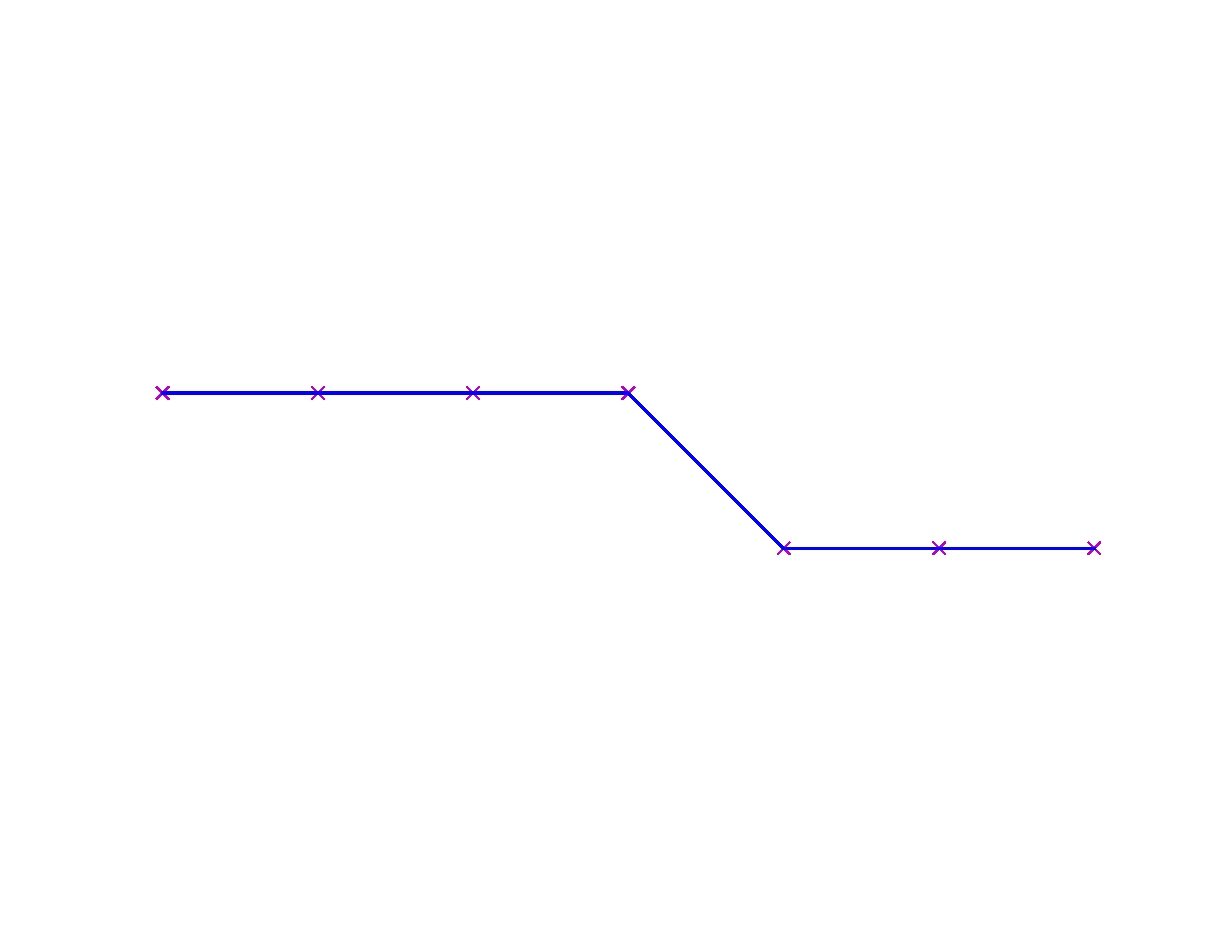
\includegraphics[width=0.45\textwidth]{spline1b}\\
\end{tabular}
\vspace*{-1cm}
\caption{(Piecewise) polynomial approximation of a rough function. Left: the Lagrange interpolant $p_6$ oscillates through the data. Right: the {\bf s}mooth {\bf p}iecewise {\bf line}ar (spline) interpolant, formed via joining consecutive data points, appears to interpolate the data more faithfully.}
\label{figure:SplineIntro}
\end{center}
\end{figure}

Given the theory we have developed for global polynomial approximation via Lagrange interpolating polynomials, it should be clear that there exists a unique solution to the interpolation problem of linear interpolating splines. Furthermore, if we start making regularity assumptions on the data, as if they were samples of a function, then we can demonstrate convergence.

\begin{theorem}\label{theorem:LinearSplineConvergence}
Let $a=x_0<x_1<\cdots<x_n=b$, and let $s(x)$ be the linear interpolating spline. Then, $s\in C([a,b])$ and it is linear on each subinterval $[x_{i-1},x_i]$, for $i=1,\ldots,n$. Let $f(x)\in C^2([a,b])$. Then:
\[
\norm{f-s}_\infty \le \dfrac{h^2}{8}\norm{f''}_\infty,
\]
where $\displaystyle h=\max_{1\le i\le n}(x_i-x_{i-1})$.
\end{theorem}
The nodes $x_i$ for $i=0,\ldots,n$ are known as the {\em knots} of the linear spline.

The linear interpolating spline $s(x)$ can be constructed by calculating slopes of data between knots and using a piecewise definition. Let:
\[
s_i(x) := f(x_{i-1}) + \dfrac{f(x_i)-f(x_{i-1})}{x_i-x_{i-1}}(x-x_{i-1}),\quad{\rm for}\quad i=1,\ldots,n.
\]
Then:
\[
s(x) := \left\{ \begin{array}{ccc}
s_1(x) & \for & x\in[x_0,x_1],\\
\vdots & \vdots & \vdots\\
s_i(x) & \for & x\in[x_{i-1},x_i],\\
\vdots & \vdots & \vdots\\
s_n(x) & \for & x\in[x_{n-1},x_n].\\
\end{array}\right.
\]
Note that we can take either the value of $s_i$ or $s_{i+1}$ at the knot $x_i$ since they are equal.

It may occur that we would like to construct piecewise polynomial interpolants with higher polynomial degree on each subinterval. It is clear that we will want our splines to continue to be interpolatory in nature, thus we will have $2n$ interpolation conditions. With piecewise linear splines, we had $2n$ unknown coefficients and these coefficients are uniquely determined. But if we use piecewise {\em quadratic} splines, then we would have $3n$ unknown coefficients and still only $2n$ interpolation conditions, and generally $(m+1)n$ unknown coefficients with piecewise splines of degree-$m$ and only $2n$ interpolation conditions.

Instead, the added unknowns in piecewise splines of higher degree allow us to enforce continuity of the interpolant, and as many of its higher order derivatives in proportion to the degree. Thus, piecewise quadratics allow for continuity of the first derivative, piecewise cubics allow for continuity of the second derivative, and so on and so forth. These continuity conditions are only applicable at the interior knots $x_1,\ldots,x_{n-1}$, and thus these conditions only give $(m-1)(n-1)$ additional conditions, where $(m-1)$ is the number of derivatives of the spline that are continuous.

Numerous methods have been proposed to add the extra conditions required to ensure that:
\[
\underbrace{(2n)}_{\hbox{interpolation}} + \underbrace{(m-1)(n-1)}_{\hbox{continuity}} + \underbrace{(m-1)}_{\hbox{extra}} = \underbrace{(m+1)n.}_{\hbox{\# degrees of freedom}}
\]

\begin{example}
Piecewise cubic interpolating splines enforce continuity in the first and second derivatives and require two extra conditions. Three common ways of fulfilling these conditions are:
\begin{enumerate}
\item specify $s'(x_0)=f'(x_0)$ and $s'(x_n) = f'(x_n)$ if derivative information is available;
\item specify $s''(x_0) = 0 = s''(x_n)$, which gives {\em natural} cubic splines; or,
\item enforce continuity of $s'''$ at $x_1$ and $x_n$, which is usually described at the ``not-a-knot'' condition\footnote{This can be reasoned because the continuity of $s'''$ implies that the first two pieces are the same cubic spline on $[x_0,x_2]$, thus $x_1$ is not a knot, and a similar argument for $x_{n-1}$.}.
\end{enumerate}
\end{example}

\begin{comment}
\subsection{B-splines}

In constructing piecewise splines of degree-$m$, one could express the splines in the monomial basis and express the $(m+1)n$ conditions in a sparse\footnote{The system will be sparse because interpolation conditions only involve one piece at a time, and the continuity conditions only involve neighbouring pieces.} linear system of equations. However, using the special {\em basis} splines (B-splines), we find even more structure.

B-splines are themselves natural piecewise polynomials but are only defined {\em locally}, with the following properties:
\[
B_{i,m}(x_i) = 1,\quad{\rm for}\quad i=m/2-1,\ldots,n-m/2+1,
\]
and $B_{i,m}(x)\equiv 0$ for $x\notin(x_{i-m+1},x_{i+m-1})$, and $\deg(B_{i,m}(x)) = m$. The first and last few B-splines have special definitions.

\begin{example}
Construction of the degree-$3$ B-spline with knots $0,1,2,3,4$. On $[0,1]$ we know that:
\[
B_{2,3}(x) = \alpha x^3,
\]
for some $a$ in order that $B_{2,3}$, $B_{2,3}'$, and $B_{2,3}''$ are all continuous at $x=0$. This implies:
\[
B_{2,3}(1) = \alpha,\quad B_{2,3}'(1) = 3\alpha,\quad{\rm and}\quad B_{2,3}''(1) = 6\alpha.
\]
On $[1,2]$, since $B_{2,3}$ is a cubic polynomial, it can be expressed as:
\begin{align*}
B_{2,3}(x) & = B_{2,3}(1) + B_{2,3}'(1)(x-1) + \dfrac{B_{2,3}''(1)}{2}(x-1)^2 + \beta(x-1)^3,\\
& = a + 3a(x-1) + 3a(x-1)^2 + \beta(x-1)^3,
\end{align*}
for some $\beta$. Since we require $B_{2,3}(2) = 1$, then $1 = 7\alpha + \beta$. Now, in order to continue, by symmetry, we must have $B_{2,3}'(2) = 0$, or:
\[
3\alpha+6\alpha + 3\beta = 9\alpha + 3 - 21\alpha = 3-12\alpha = 0,
\]
or $\alpha = \tfrac{1}{4}$ and $\beta = -\tfrac{3}{4}$. Thus:
\[
B_{2,3}(x) = \left\{\begin{array}{ccc}
0 & \for & x<0,\\
\frac{1}{4}x^3 & \for & x\in[0,1],\\
\frac{1}{4} + \frac{3}{4}(x-1) + \frac{3}{4}(x-1)^2 - \frac{3}{4}(x-1)^3 & \for & x\in[1,2],\\
\frac{1}{4} + \frac{3}{4}(3-x) + \frac{3}{4}(3-x)^2 - \frac{3}{4}(3-x)^3 & \for & x\in[2,3],\\
\frac{1}{4}(4-x)^3 & \for & x\in[3,4],\\
0 & \for & x>4.
\end{array}\right.
\]
\end{example}
\end{comment}

\section{Problems}
\begin{enumerate}
\item Theorems~\ref{theorem:polyexistence} and~\ref{theorem:polyuniqueness} establish existence and uniqueness of polynomial interpolants with distinct absciss\ae~via Lagrange interpolating polynomials and the Fundamental Theorem of Algebra. An alternative proof relies on expressing any polynomial in the monomial basis:
\[
p_n(x) = \sum_{k=0}^n c_k x^k.
\]
Then, since any interpolating polynomial must satisfy the linear system $Ac = f$:
\begin{equation}\label{eq:Aceqf}
\begin{bmatrix}
1 & x_0 & x_0^2 & \cdots & x_0^n\\
1 & x_1 & x_1^2 & \cdots & x_1^n\\
1 & x_2 & x_2^2 & \cdots & x_2^n\\
\vdots & \vdots & \vdots & \ddots & \vdots\\
1 & x_n & x_n^2 & \cdots & x_n^n\\
\end{bmatrix}
\begin{bmatrix}
c_0\\c_1\\c_2\\\vdots\\c_n
\end{bmatrix}
=
\begin{bmatrix}
f_0\\f_2\\f_3\\\vdots\\f_n
\end{bmatrix},
\end{equation}
for the existence and uniqueness of $p_n$ it suffices to show that $\det(A)\ne0$. Prove that:
\[
\det(A) = \prod_{i=1}^n\prod_{j=0}^{i-1} (x_i-x_j).
\]

\item Na\"ively, one might expect to obtain a formula for the error of the derivative of the Lagrange interpolating polynomial $f'-p_n'$. However, it is not clear that $\xi = \xi(x)$ in Theorem~\ref{theorem:LagrangeInterpolatingRemainder} is even differentiable. An alternative approach leads to the following formula. Prove (and state conditions) that there exist distinct points $z_i\in(x_i,x_{i+1})$ for $i=0,\ldots,n-1$ such that:
\[
\rho_n(x) := f'(x) - p_n'(x) = \dfrac{f^{(n+1)}(\eta)}{n!}\prod_{i=0}^{n-1}(x-z_i),
\]
for some $\eta\in(a,b)$ and for each $x\in[a,b]$. {\em Hint: take the error formula $r(x)$ in Theorem~\ref{theorem:LagrangeInterpolatingRemainder}, and apply the Mean Value Theorem on each sub-interval $[x_i,x_{i+1}]$ for $i=0,\ldots,n-1$. This gives you the $n$ points $z_i$ where $f'(z_i) - p_n'(z_i) = 0$.}
\item It is sometimes possible to obtain explicit formul\ae~for the barycentric weights $\lambda_k$. Show that for the equispaced nodes in $[-1,1]$, $x_k = -1 + 2k/n$ for $k=0,\ldots,n$, the barycentric weights are:
\[
\lambda_k = \dfrac{(-\tfrac{n}{2})^n}{n!}\binom{n}{k}(-1)^k.
\]
Why may we discard the first part, depending only on $n$, and use the modified weights:
\[
\tilde{\lambda}_k = \binom{n}{k}(-1)^k,
\]
in the second barycentric formula?
\begin{comment}
\item The (symmetrically truncated) cardinal series of a function $f$ is defined by:
\[
C_n(f,h)(x) = \sum_{k=-n}^n f(kh) \sinc\left(\dfrac{x-kh}{h}\right),
\]
where $h>0$ is the spacing of the data and the $\sinc$ function is defined by:
\[
\sinc(x) := \left\{\begin{array}{ccc} \dfrac{\sin(\pi x)}{\pi x}, & \for & x\ne 0,\\ 1, & \for & x = 0.\end{array}\right.
\]
Under appropriate conditions, $C_n(f,h)(x)$ approximates $f(x)$ on $[-nh,nh]$.
\begin{enumerate}
\item Show that:
\[
C_n(f,h)(x) = \dfrac{h}{\pi}\sin\dfrac{\pi x}{h}\sum_{k=-n}^n \dfrac{(-1)^k}{x-kh}f(kh),
\]
or the first barycentric formula for the cardinal series. Since this requires the evaluation of only one value of the sine function, it provides a more efficient way to evaluate the cardinal series that by definition.
\item If instead of approximating $f$ we approximate the weighted function $wf$, where $w>0$, we obtain the modified cardinal series:
\[
C_n(f,h,w)(x) = \dfrac{1}{w(x)}\sum_{k=-n}^n w_kf(kh) \sinc\left(\dfrac{x-kh}{h}\right),
\]
where $w_k = w(kh)$. Under certain conditions on $w$, we may still expect to approximate $f(x)$ on $[-nh,nh]$ by $C_n(f,h,w)(x)$. Use a cardinal series for $w$ to show that:
\[
C_n(f,h,w)(x) \approx \dfrac{\displaystyle\sum_{k=-n}^n \dfrac{(-1)^kw_k}{x-kh}f(kh)}{\displaystyle\sum_{k=-n}^n \dfrac{(-1)^kw_k}{x-kh}}.
\]
This is the second barycentric formula for the cardinal series. It reduces approximation by cardinal series to a rational approximation of $f$.
\item Write a program to approximate $f(x) = \dfrac{1}{1+e^x}$ with a cardinal series on the interval $[-10,10]$ using the weight function $w(x) = e^{-x^2}$.
\end{enumerate}
\end{comment}
\item Generalize Horner's rule for numerical evaluation of polynomials in the monomial basis to numerical evaluation of polynomial interpolants in Newton form.
%\item Under what conditions on the inner product space $L^2(D,w(x)\ud x)$ are even-degree orthogonal polynomials even and odd-degree orthogonal polynomials odd?
\item The Chebyshev expansion of a function $f\in L^2(\I,(1-x^2)^{-\frac{1}{2}}\ud x)$ is determined by:
\[
f(x) \sim \sum_{n=0}^\infty c_n T_n(x),\quad{\rm where}\quad c_n = \dfrac{\langle T_n, f\rangle}{\langle T_n, T_n\rangle}.
\]
In some instances, Chebyshev expansions are known in closed form, such as:
\[
f(x) = \dfrac{1}{x^2+a^2} \sim \dfrac{1}{a\sqrt{a^2+1}}\left(1+2\sum_{n=1}^\infty\dfrac{(-1)^n}{(a+\sqrt{a^2+1})^{2n}}T_{2n}(x)\right),\quad{\rm for}\quad a>0.
\]
\begin{enumerate}
\item Show that:
\[
\langle T_0,T_0\rangle = \pi,\quad{\rm and}\quad \langle T_n,T_n\rangle = \dfrac{\pi}{2},\quad{\rm for}\quad n\in\N.
\]
\item Calculate $\norm{f}_{\infty}$ and $\norm{f}_{2,w}$, the weighted $2$-norm associated with $L^2(\I,(1-x^2)^{-\frac{1}{2}}\ud x)$. {\em Hint: for the weighted $2$-norm, use the Chebyshev expansion and orthogonality of the Chebyshev polynomials.}
\item Let $p_N(x)$ denote the degree-$N$ Chebyshev expansion of $f$.
Which $N( = N(a,\varepsilon))$ is required to satisfy:
\[
\norm{f-p_N}_{2,w} \le \varepsilon\norm{f}_{2,w}?
\]
\item Which $N( = N(a,\varepsilon))$ is required to satisfy:
\[
\norm{f-p_N}_\infty \le \varepsilon\norm{f}_\infty?
\]
\end{enumerate}

\item Calculate the first five orthogonal polynomials with respect to $L^2([-1,-a]\cup[a,1],\ud x)$ for some $a\in[0,1)$. While inapplicable, Theorem~\ref{theorem:OPzeros} makes a statement on the locii of the zeros of orthogonal polynomials with respect to $L^2([a,b],\ud\mu(x))$ for some monotonic measure $\mu$. Can anything be said about the locii of the zeros in the current case? What do you expect when $\lim_{a\to0}\pi_n(x;a)$?
\item Prove Theorem~\ref{theorem:LinearSplineConvergence}.
\end{enumerate}